\documentclass[a4paper, 12pt, oneside]{report}

\setcounter{tocdepth}{3}
\setcounter{secnumdepth}{3}
\usepackage{fontspec}
\usepackage{float}
\setmainfont{Times New Roman}
% \usepackage[style = authoryear]{biblatex}
% \addbibresource{references.bib}
\usepackage{setspace}
\doublespace 
\usepackage{lipsum}
\usepackage{graphicx}
\graphicspath{{figures/}}
% \usepackage{booktabs}
\usepackage{cite}

\usepackage{geometry} % 导入geometry宏包
\geometry{top=2.54cm, bottom=2.54cm, left=2.54cm, right=2.54cm}

\setstretch{1}
\setlength{\parindent}{0pt}
\setlength{\parskip}{0.5em}

\usepackage{tocloft}
\renewcommand{\cftchapdotsep}{\cftdotsep} % 让章节后有点
\renewcommand{\cftsecdotsep}{\cftdotsep}  % 让小节后有点
\setlength{\cftbeforechapskip}{20pt} % 设置章节前的间距
\setlength{\cftbeforesecskip}{10pt}  % 设置小节前的间距

\usepackage{titlesec}
\titlespacing*{\chapter}{0pt}{0pt}{10pt} % 章节 {左边距}{上间距}{下间距}
\titleformat{\chapter}[display]
  {\normalfont\huge\bfseries} % 标题字体
  {\appendixname\ \thechapter} % 附录标签格式
  {10pt} % 标签与标题之间的距离
  {\Huge} % 标题字体大小

\usepackage{amsmath}
\usepackage{amsfonts}

  % 定义新的section命令,带有数字编号但没有章节号
% \newcommand{\customsection}[1]{%
%     \refstepcounter{section}% 递增section计数器
%     \section*{\thesection\quad #1}% 显示数字编号和标题
%     \addcontentsline{toc}{section}{\protect\numberline{}#1}% 添加到目录
% }
\usepackage{graphicx} % 用于插入图形
\usepackage{caption}   % 用于自定义标题样式
% 设置所有图形标题为斜体
\captionsetup{font=it}
\captionsetup{justification=centering}

\begin{document}

\thispagestyle{empty}
\begin{center}

\begin{figure}
    \centering
    
\includegraphics[width=0.75\linewidth]{figures/PolyU.png}
\end{figure}


\LARGE

\textbf{The Hong Kong Polytechnic University \\
Department of Mechanical Engineering \\
Final Year Project: Interim Report \\}
\vspace{1cm}
\textbf{Development of Deep Learning Approaches for Sound Source Localization (SSL)}
\vspace{1cm}

Group 22\\
\vspace{1cm}
ZENG Bailin (21107431D)\\
WU Zhuoli (21103602D)\\
XIAO Pengbo (21107461D)




\end{center}
\pagenumbering{roman}
% \chapter*{Publications arising from the thesis}

\bigskip

\begin{refsection}
\nocite{doe2020publication, doe2021another}

\printbibliography[heading = none]
\end{refsection}

\tableofcontents
% \listoffigures
% \listoftables

\pagenumbering{arabic}
\chapter*{Introduction}
\addcontentsline{toc}{chapter}{Introduction}

Audio processing involves the manipulation and analysis of sound signals to enhance, modify, or analyze the audio data. This incorporates a wide range of techniques and algorithms. The types of audio signals categorize the audio processing into analog and digital processing. In the context of sound source localization, the settings mostly refer to the digital audio signal analysis.

Sound source localization (SSL) is the process of identifying the relative location of one or multiple sound sources in a given environment with various acoustic signals \cite{desai_review_2022}. This technique plays a significant role in acoustic signal processing, enabling the system to interpret the audio information spatially.

\begin{figure}[h]
    \centering
    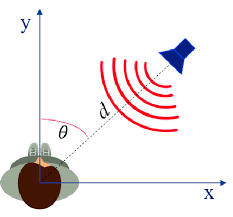
\includegraphics[width=0.3\linewidth]{figures/SSL_Explain.png}
    \caption{Principle of SSL}
    % \label{fig:enter-label}
\end{figure}

The SSL methods mostly utilize a microphone array that contains multiple microphones for source localization purposes, which is similar to other signal positioning systems, the Global Navigation Satellite System (GNSS) as an example, and is hardly achievable by using a single signal receiver. In this project, the SSL process will be conducted using a multi-microphone array.

\begin{figure}[h]
    \centering
    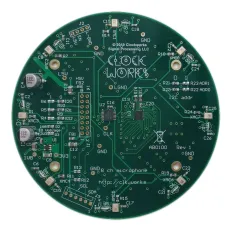
\includegraphics[width=0.3\linewidth]{figures/Microphone_Array1.png}
    \caption{An Example of 8-Channels Microphone Array}
    % \label{fig:enter-label}
\end{figure}

When considering the transmission of sound waves in space, the process can usually be described by two different models: the near-field model and the far-field model \cite{westervelt_parametric_1963}. The near-field model refers to scenarios where the distance between the sound source and the microphone array is short, resulting in sound waves being treated as spherical waves. Conversely, the far-field model applies when the distance is sufficiently large to consider the sound waves as plane waves. In the following studies, the far-field condition will be applied to all situations.

Traditionally, the SSL problems can be resolved in various ways. These methods typically estimate the direction of arrival (DoA) of the sound signal using mathematical models. However, limitations exist among these methods. For example, conventional approaches like multiple signal classification (MUSIC) have limitations in processing overlapping sound sources and noisy scenarios \cite{limitation_MUSIC_2021}.

\begin{figure}[h]
    \centering
    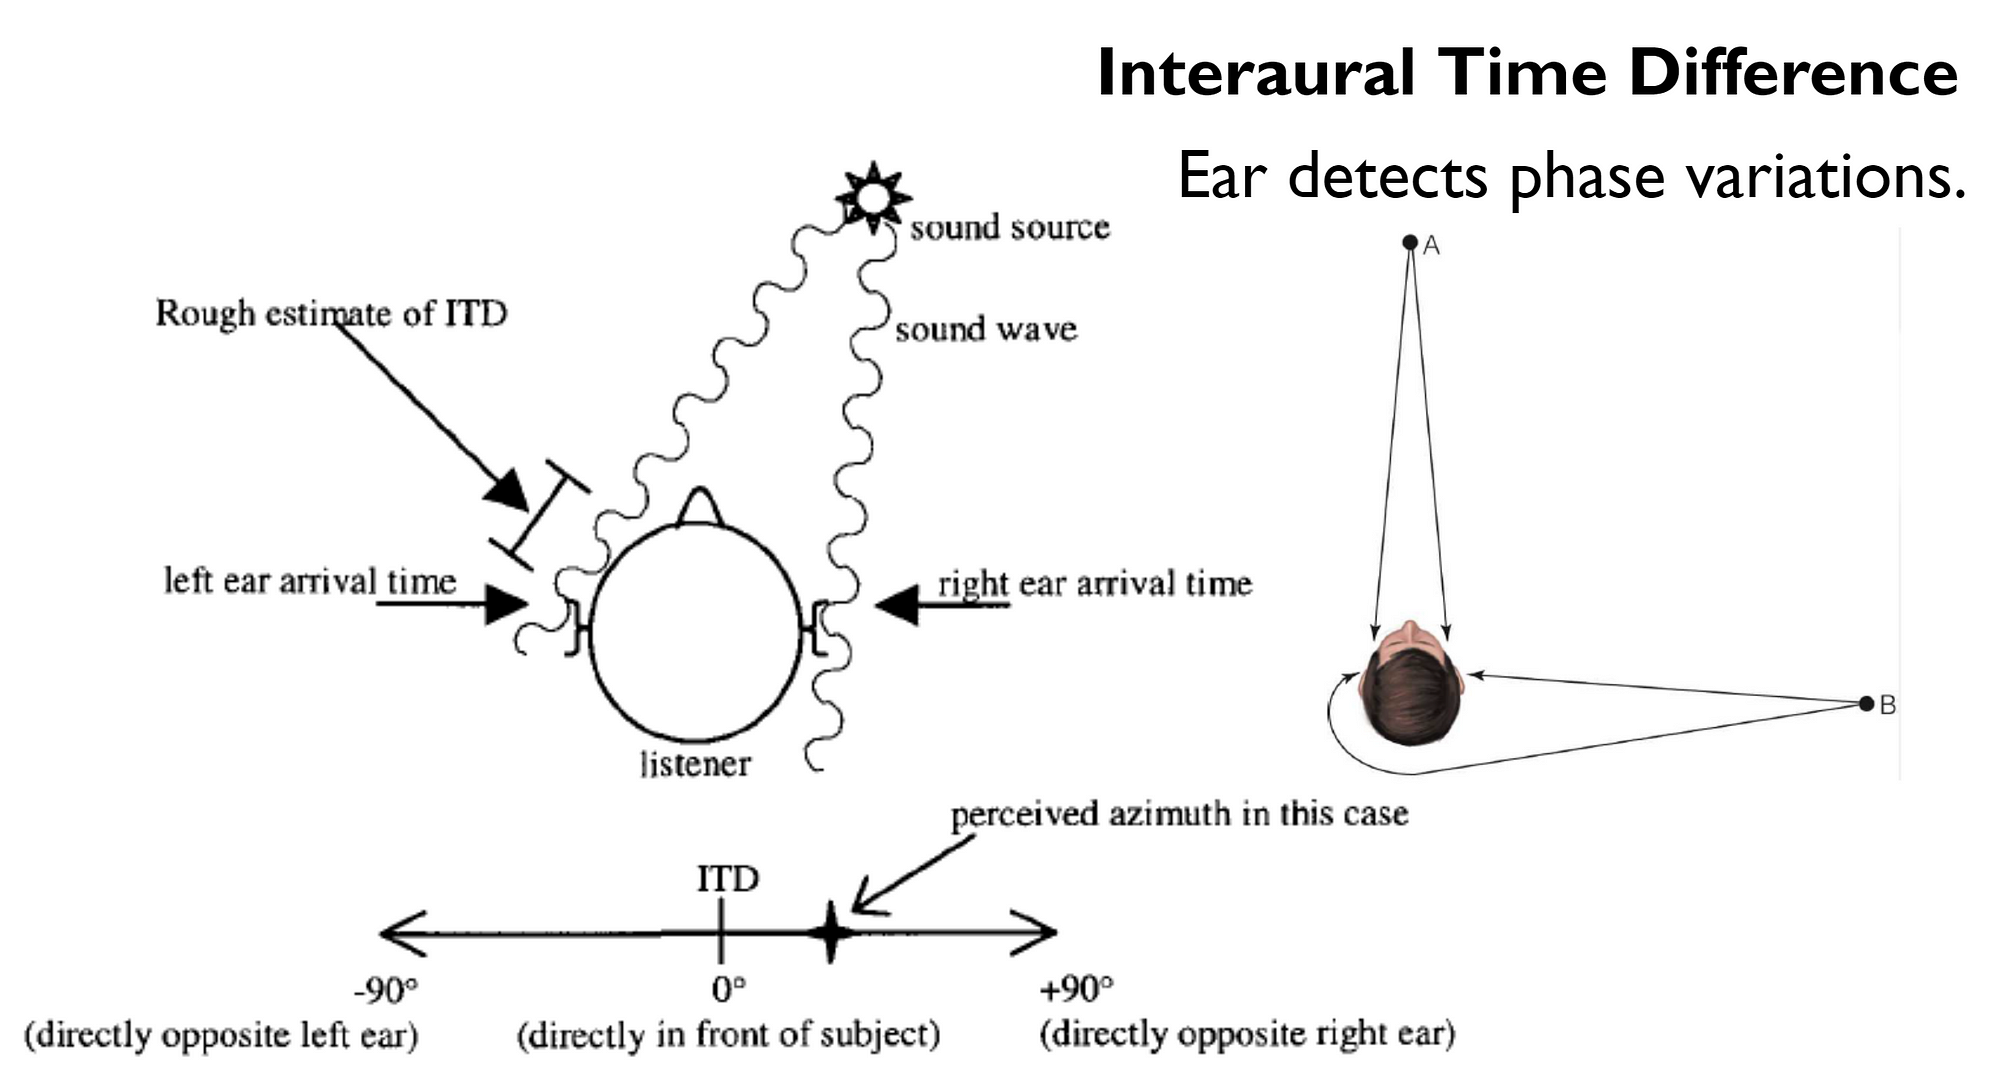
\includegraphics[width=0.5\linewidth]{figures/Human_Ears_TDOA.png}
    \caption{Human Ears Provide a Typical Example of TDOA}
    % \label{fig:enter-label}
\end{figure}

In recent years, deep learning (DL) has emerged as a branch of machine learning, being an innovative solution to robot perceptual problems. By utilizing large datasets and neural network architectures, deep learning models, often referred to as deep neural networks (DNN), can extract relevant information and features from the original audio signals, either directly or indirectly, without the need of physical-meaning-based mathematical models. DL techniques such as convolutional neural networks (CNNs) and recurrent neural networks (RNNs) have already demonstrated promising results in the audio processing area, overcoming several limitations in the traditional algorithms such as the noise and reverberation problems in a given environment.

 One of the most significant SSL applications is robotic perception since understanding the location of sounds can enhance robots' navigation capabilities, especially for non-stationary obstacle identification abilities. However, different from the situation of SSL in the laboratory context, SSL perception for robots requires high robustness, computational efficiency, and adaptivity to complex environments.





















% \section{Section}
% \subsection{Subsection}
% \subsubsection{Subsubsection}
% \lipsum[1-5] \parencite{cicero1883finibus}

% \begin{figure}[ht]
%     \centering
%     
\includegraphics[width = 0.5\textwidth]{PolyU.png}
%     \caption{The Hong Kong Polytechnic University}
%     \label{PolyU}
% \end{figure}

% \begin{table}[ht]
%     \centering
%     \begin{tabular}{l|l}
%     \toprule
%          This & is \\ \midrule
%          a & table.\\ \bottomrule
%     \end{tabular}
%     \caption{A table}
%     \label{Table}
% \end{table}


\chapter*{Goal, Objectives and Project Plan}
\addcontentsline{toc}{chapter}{Goal, Objectives and Project Plan}

In this Final Year Project (FYP), the goal is to develop an advanced DL-based method for SSL and explore the possibilities of deploying the DNN on a mobile platform for real-time SSL.

The objectives of this project are to:
\begin{enumerate}
    \item Investigate the mathematical-model-based traditional SSL approaches by reproducing the experiment of SSL using these algorithms, establishing standards for the development of DNN.
    \item Conduct research on the performance of the state-of-the-art DNNs' architectures, reproducing the DoA estimation process of these DNNs by using the computationally generated dataset.
    \item Develop an accurate DNN structure to predict the location of a stationary sound source and further develop a DNN structure for real-time sound source trajectory tracking.
    \item Develop a mobile platform based on the Robot Operating System (ROS) and develop the software program for the deployment of newly developed SSL approaches, enabling the platform to react to the sound source.
    \item Conduct field tests using the real-world audio data to evaluate the performance of the DL approaches and conduct experiments to evaluate the mobile platform's performance regarding a sound source.
\end{enumerate}

These objectives are categorized into three parts: the traditional SSL algorithm, the DL-based SSL algorithm, and the mobile platform. These parts are assigned to XIAO Pengbo, ZENG Bailin, and WU Zhuoli, respectively. The detailed schedule of this FYP is described in \textit{the Gantt Chart for Task Schedule} section of the appendices.




\chapter*{Literature Review}
\addcontentsline{toc}{chapter}{Literature Review}

Related works of SSL are categorized into two sections, the traditional SSL methods and the DL based SSL approaches.

\section*{Review of Traditional SSL Methods}
\addcontentsline{toc}{section}{Review of Traditional SSL Methods}

Traditional Sound Source Localization (SSL) methods primarily rely on mathematical modeling of geometric and statistical principles. These approaches employ a variety of techniques to estimate the locations of sound sources within an environment. These foundational methods have established foundations for more sophisticated SSL techniques and remain crucial in various audio signal processing applications.

A typical traditional SSL method is the Time Difference of Arrival (TDOA) \cite{knapp_generalized_1976}. It positions the spatial location of a sound source by measuring the time differences of the sound signal arrival time between each microphone in a microphone array. With two microphones, the TDOA method can position the degree of arrival (DoA) of the sound source relative to the receiver, while three or more microphones can position the DoA and distance by triangulate positioning. TDOA methods have been progressively improved over the decades to adapt to various scenarios such as when the number of microphones is limited \cite{liu_arbitrary_2019} or when sound wave transmission mediums are different \cite{carevic_detection_2007}. Combining the TDOA method with other statistical models is also a research trend, combined with Generalized Cross-Correlation (GCC) \cite{chung_sound_2022} as an example. However, multiple research claimed that the TDOA method is limited when encountering situations such as high noise levels, low noise-signal ratio, and reverberant environment \cite{tachioka_method_2017} \cite{hao_network_2020}.

Another widely used classical algorithm is beamforming \cite{van_veen_beamforming_1988}. By employing microphone arrays to enhance signals coming from specific directions while suppressing signals from other directions, it scans all possible directions, and the direction with the maximum gain (main lobes) is estimated as the direction of the sound source. As another classical SSL approach, beamforming was utilized for various purposes. Based on beamforming methods, researchers proposed effective solutions to blind sound source separation based on geometric beam-forming \cite{parra_geometric_2002}. It was also proven to have the potential to be applied to robotic perception \cite{valin_localization_2004}. However, there is also a concern about the beamforming algorithm's performance in complex situations, including localizing non-stationary background noise \cite{comminiello_beamforming_2013}, and reverberant environment \cite{noh_dereverberation_2020}.

\begin{figure}[H]
    \centering
    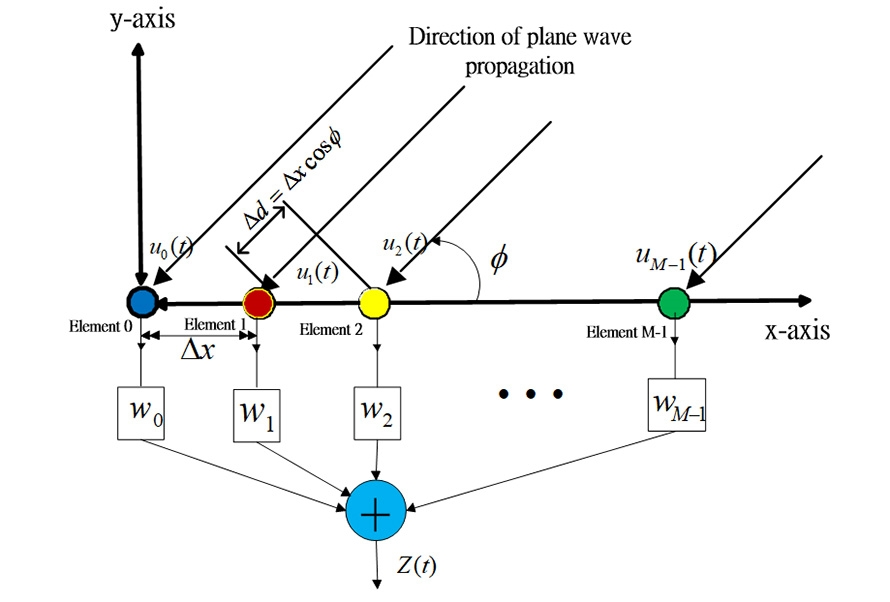
\includegraphics[width=0.4\linewidth]{figures/Explain_beamforming.png}
    \caption{Beamforming Utilizes Phase Shift to Enhance the Signal from the Scanned Direction}
\end{figure}


\section*{Review of Deep-Learning Based SSL Methods}
\addcontentsline{toc}{section}{Review of Deep-Learning Based SSL Methods}

With advancements in GPU technology and its computational capabilities during the last decade, the growing complexity of DNN architecture provides possibilities to improve the accuracy and robustness of the SSL. Recent studies demonstrate the robustness of DL-based SSL algorithms under noisy and reverberant environments \cite{wang_robust_2018} \cite{zhang_deep_2017} \cite{lee_sound_2020} \cite{ma_exploiting_2017}. The robustness of these algorithms while handling complex circumstances enables them to be deployed in a wider range of applications, with Unmanned Aerial Vehicle (UAV) \cite{wang_deep-learning-assisted_2022} as an example.

Most of the DL-based approaches for SSL purposes involve five stages: pre-processing, encoding, hidden layer processing, decoding, and post-processing.

Pre-processing refers to the data processing sequence before entering the DNN, usually referring to the feature extraction algorithm that directly handles the original sound signal, which is the amplitude-time sequential data. For an audio signal processing task, feature extraction usually maps the time-domain signal to the frequency domain. A significant number of machine-learning-based methods utilize the Mel-Frequency Cepstral Coefficients (MFCCs) method, such as \cite{di_applicability_2023} \cite{nsalo_kong_underwater_2024} \cite{palaniappan_comparative_2014} \cite{wang_research_2024}, for frequency-domain information extraction and the purpose of comprehending the human speaking sound. The Fourier Transform (FT), as part of the MFCCs method, projects the sound signal from the time domain to the frequency domain, allowing a more detailed analysis of the frequency features. Another commonly employed feature extraction technique is the Short-Time Fourier Transform (STFT), which retains time-domain information by applying the Fourier Transform to each time frame instead of the entire sound signal segment. This results in a spectrogram in the time-frequency domain, including the information along the time sequence. The STFT has been increasingly utilized recently as feature extraction for DNN, with examples including \cite{tan_sound_2021} 
\cite{chakrabarty_multi-speaker_2019} \cite{pujol_beamlearning_2021} \cite{schymura_pilot_2021} \cite{niu_deep-learning_2019} \cite{liu_rolling_2016}, due to its unique ability to handle time-sequential information. Meanwhile, some studies suggest that eliminating the feature extraction process, allowing the DNN to process the original time-domain sound signal directly, may yield improved performance. TasNet \cite{luo_tasnet_2018}, as an important study that resolves the audio channel separation problem by directly inputting the original multi-channel input into the DNN.

\begin{figure}[h]
    \centering
    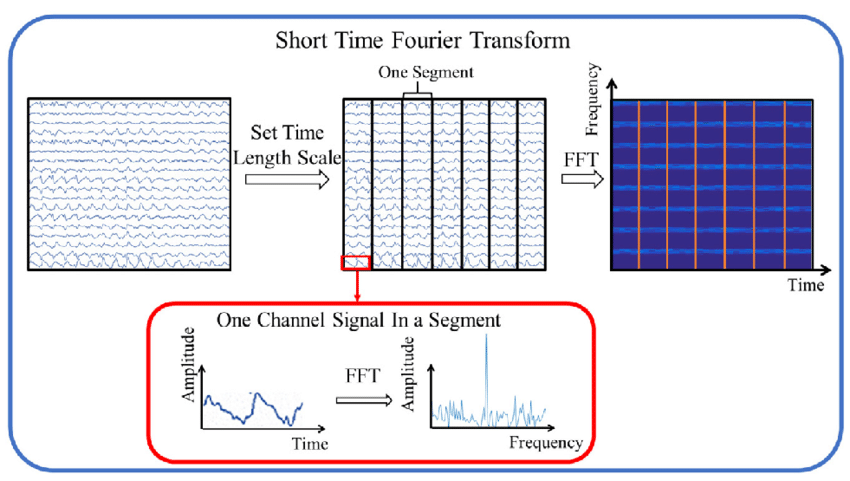
\includegraphics[width=0.75\linewidth]{figures/STFT_Explain.png}
    \caption{STFT: Applying Fourier Transform to Each Time Frame}
\end{figure}

The structures in the Deep Neural Networks (DNNs) consist of the encoder, hidden layer, and decoder. The fundamental concept of a DNN is to vectorize abstract features from the original dataset, construct a high-dimensional function (which predicts the expected output from input) described by the network itself, and compute the parameters in this function by repeated training using massive data with labeled ground truth. The training process usually refers to using gradient descent to find a local stable point in this function. In this context, the encoder refers to the mapping process from data to high-dimensional tensors for the DNN. The hidden layers serve as the prediction function. The decoder then translates the output tensors into the output required by the algorithm.

\begin{figure}[h]
    \centering
    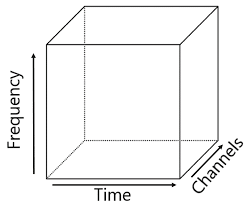
\includegraphics[width=0.25\linewidth]{figures/STFT_Tensor.png}
    \caption{The Time-Frequency Domain Spectrogram After STFT, Represented in the Form of A Tensor for Multi-Microphone-Channels Signal}
\end{figure}

\begin{figure}[h]
    \centering
    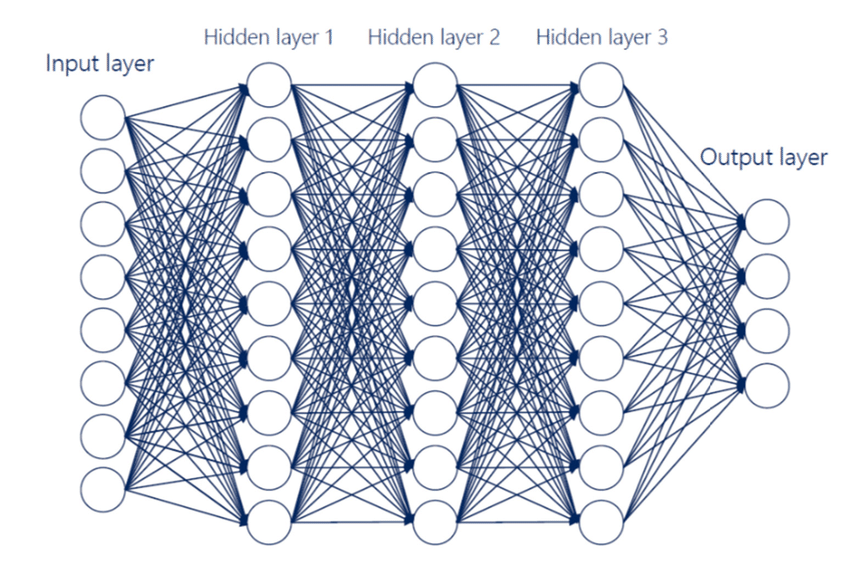
\includegraphics[width=0.5\linewidth]{figures/DNN_example2.png}
    \caption{A Simple Visualization of a Typical DNN}
\end{figure}

Whether post-processing is necessary depends on the specific settings of the SSL task. It is common for a DNN to directly output results, such as the locations of multiple sound sources in the form of a set of vectors or a time-sequence of coordinates representing the sound source's location, such as \cite{adavanne_sound_2019} \cite{zhang_mtf-crnn_2020} \cite{phan_robust_2016} \cite{kim_multi-scale_2022}. Alternatively, designing the DNN to output results to a traditional algorithm, known as post-processing, is another possible structural solution. SRP-DNN \cite{yang_srp-dnn_2022} is a suggestive example of utilizing DNN to predict the phase difference between a pair of microphones in a microphone array, which will be further constructed into a spatial spectrum for peak analysis, providing the result of the sound location.

\chapter*{Methodology}
\addcontentsline{toc}{chapter}{Methodology}

In this section, the scenario setting of the project will be defined, and the theoretical methodology of the traditional SSL algorithm, DL-based SSL algorithm, and mobile platform will be described. The definition of the scenario setting is crucial for the purpose of research since different settings require different solutions. \\


The microphone array setting is tentatively described by the following:
\begin{enumerate}
    \item A hexagonal-shaped microphone array consists of six chip microphones, placed on a hexagonal 3D-printed foundation.
    \item The microphone center is defined as located at the origin of the microphone array coordinate system.
    \item The distance between the array center and each microphone is \(0.06m\).
    \item The geometry of the microphone array is shown below:
    \begin{figure}[H]
        \centering
        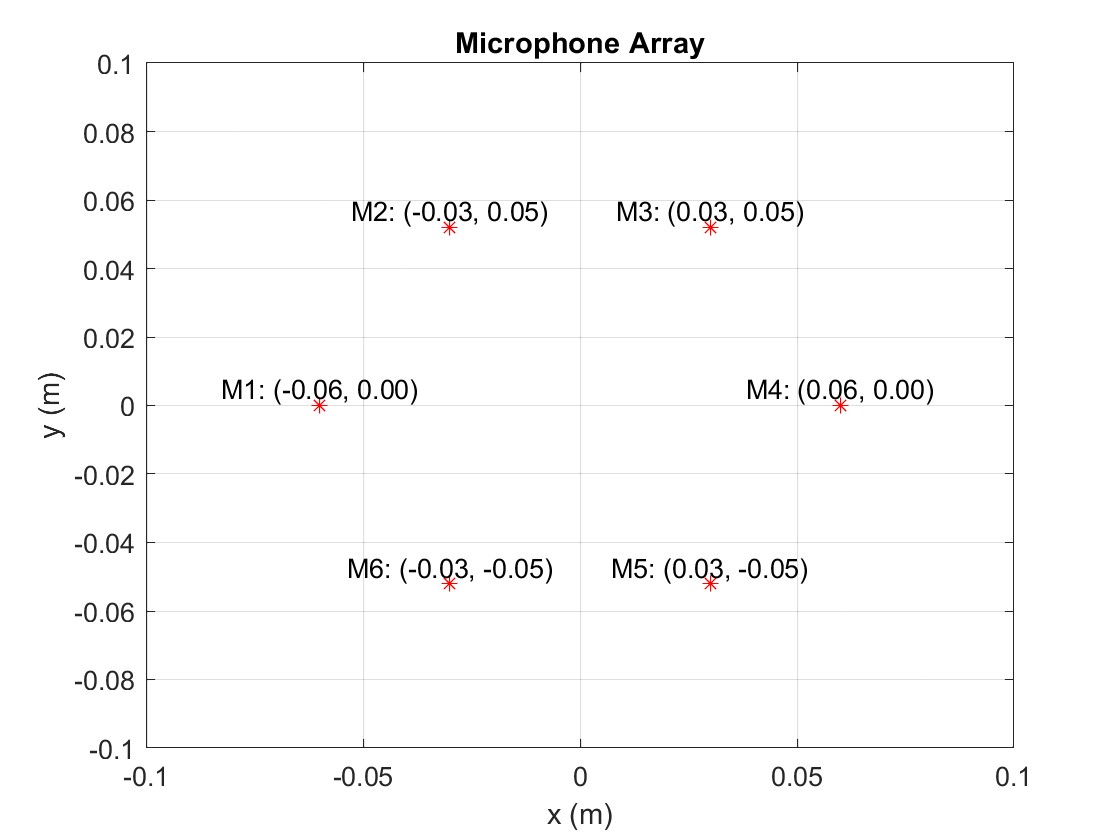
\includegraphics[width=0.8\linewidth]{figures/Geometry_microphone_array.jpg}
        \caption{The Geometry of the Hexagonal Microphone Array}
    \end{figure}
    \item The six microphones in the array are connected to a pre-processing PCB board which serves to combine the six channels signals into a USB serial port and to provide a buffer for the data. The apparatus of the microphone array is demonstrated below: 
    \begin{figure}[H]
        \begin{minipage}{0.45\textwidth}
                \centering
                \rotatebox[origin=c]{90}{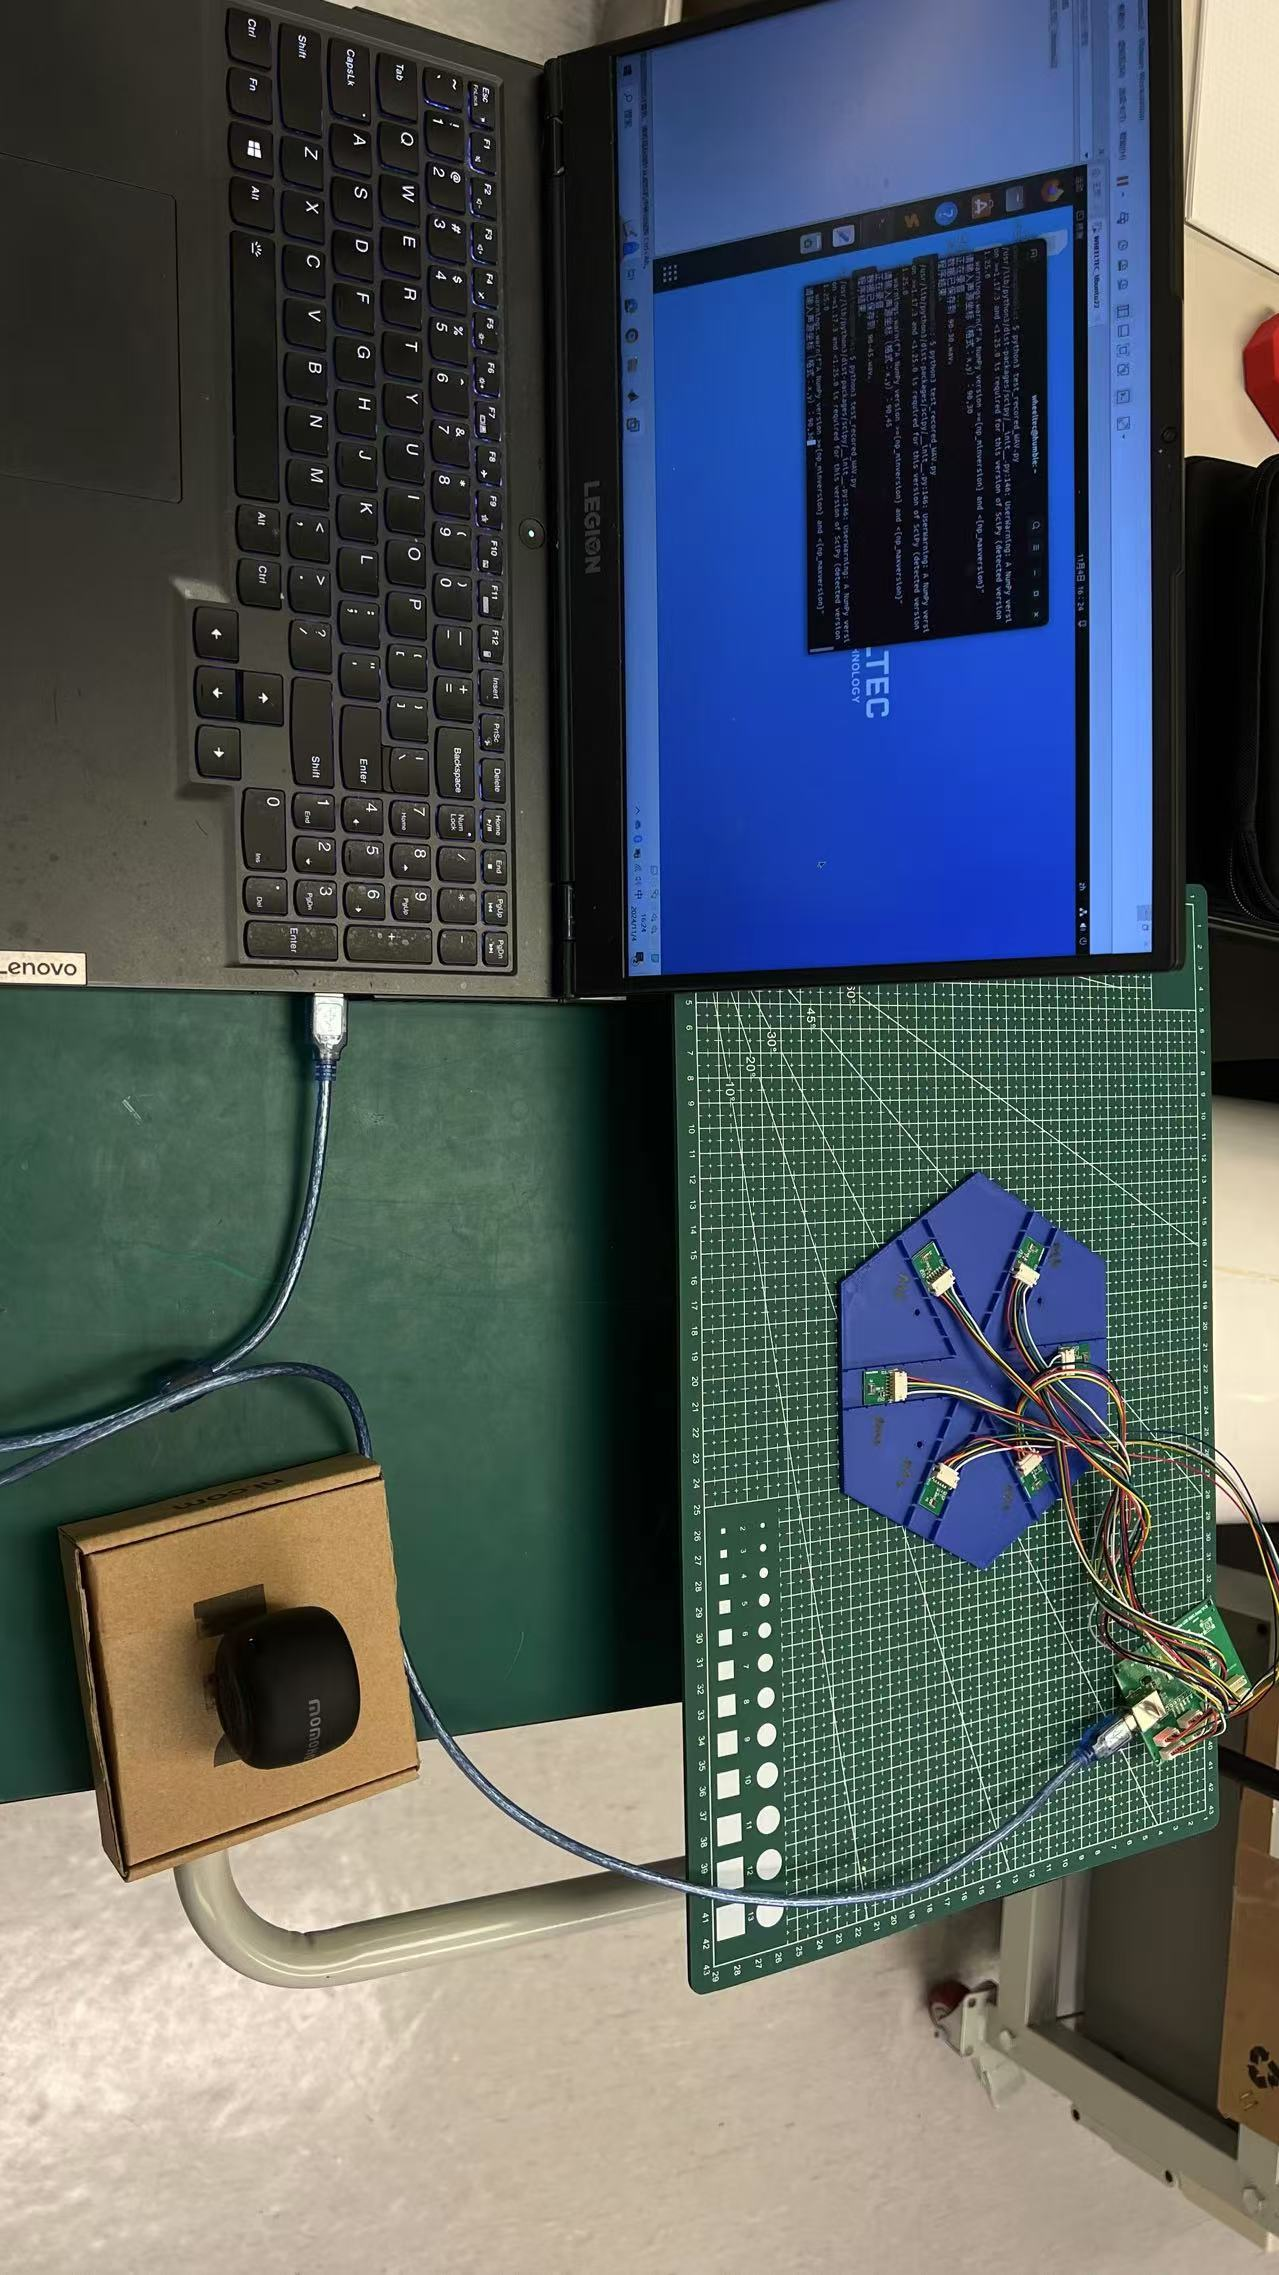
\includegraphics[width=0.5\linewidth]{figures/Microphone_array_photo.jpg}}
        \end{minipage}
        \begin{minipage}{0.45\textwidth}
                \centering
                \rotatebox[origin=c]{90}{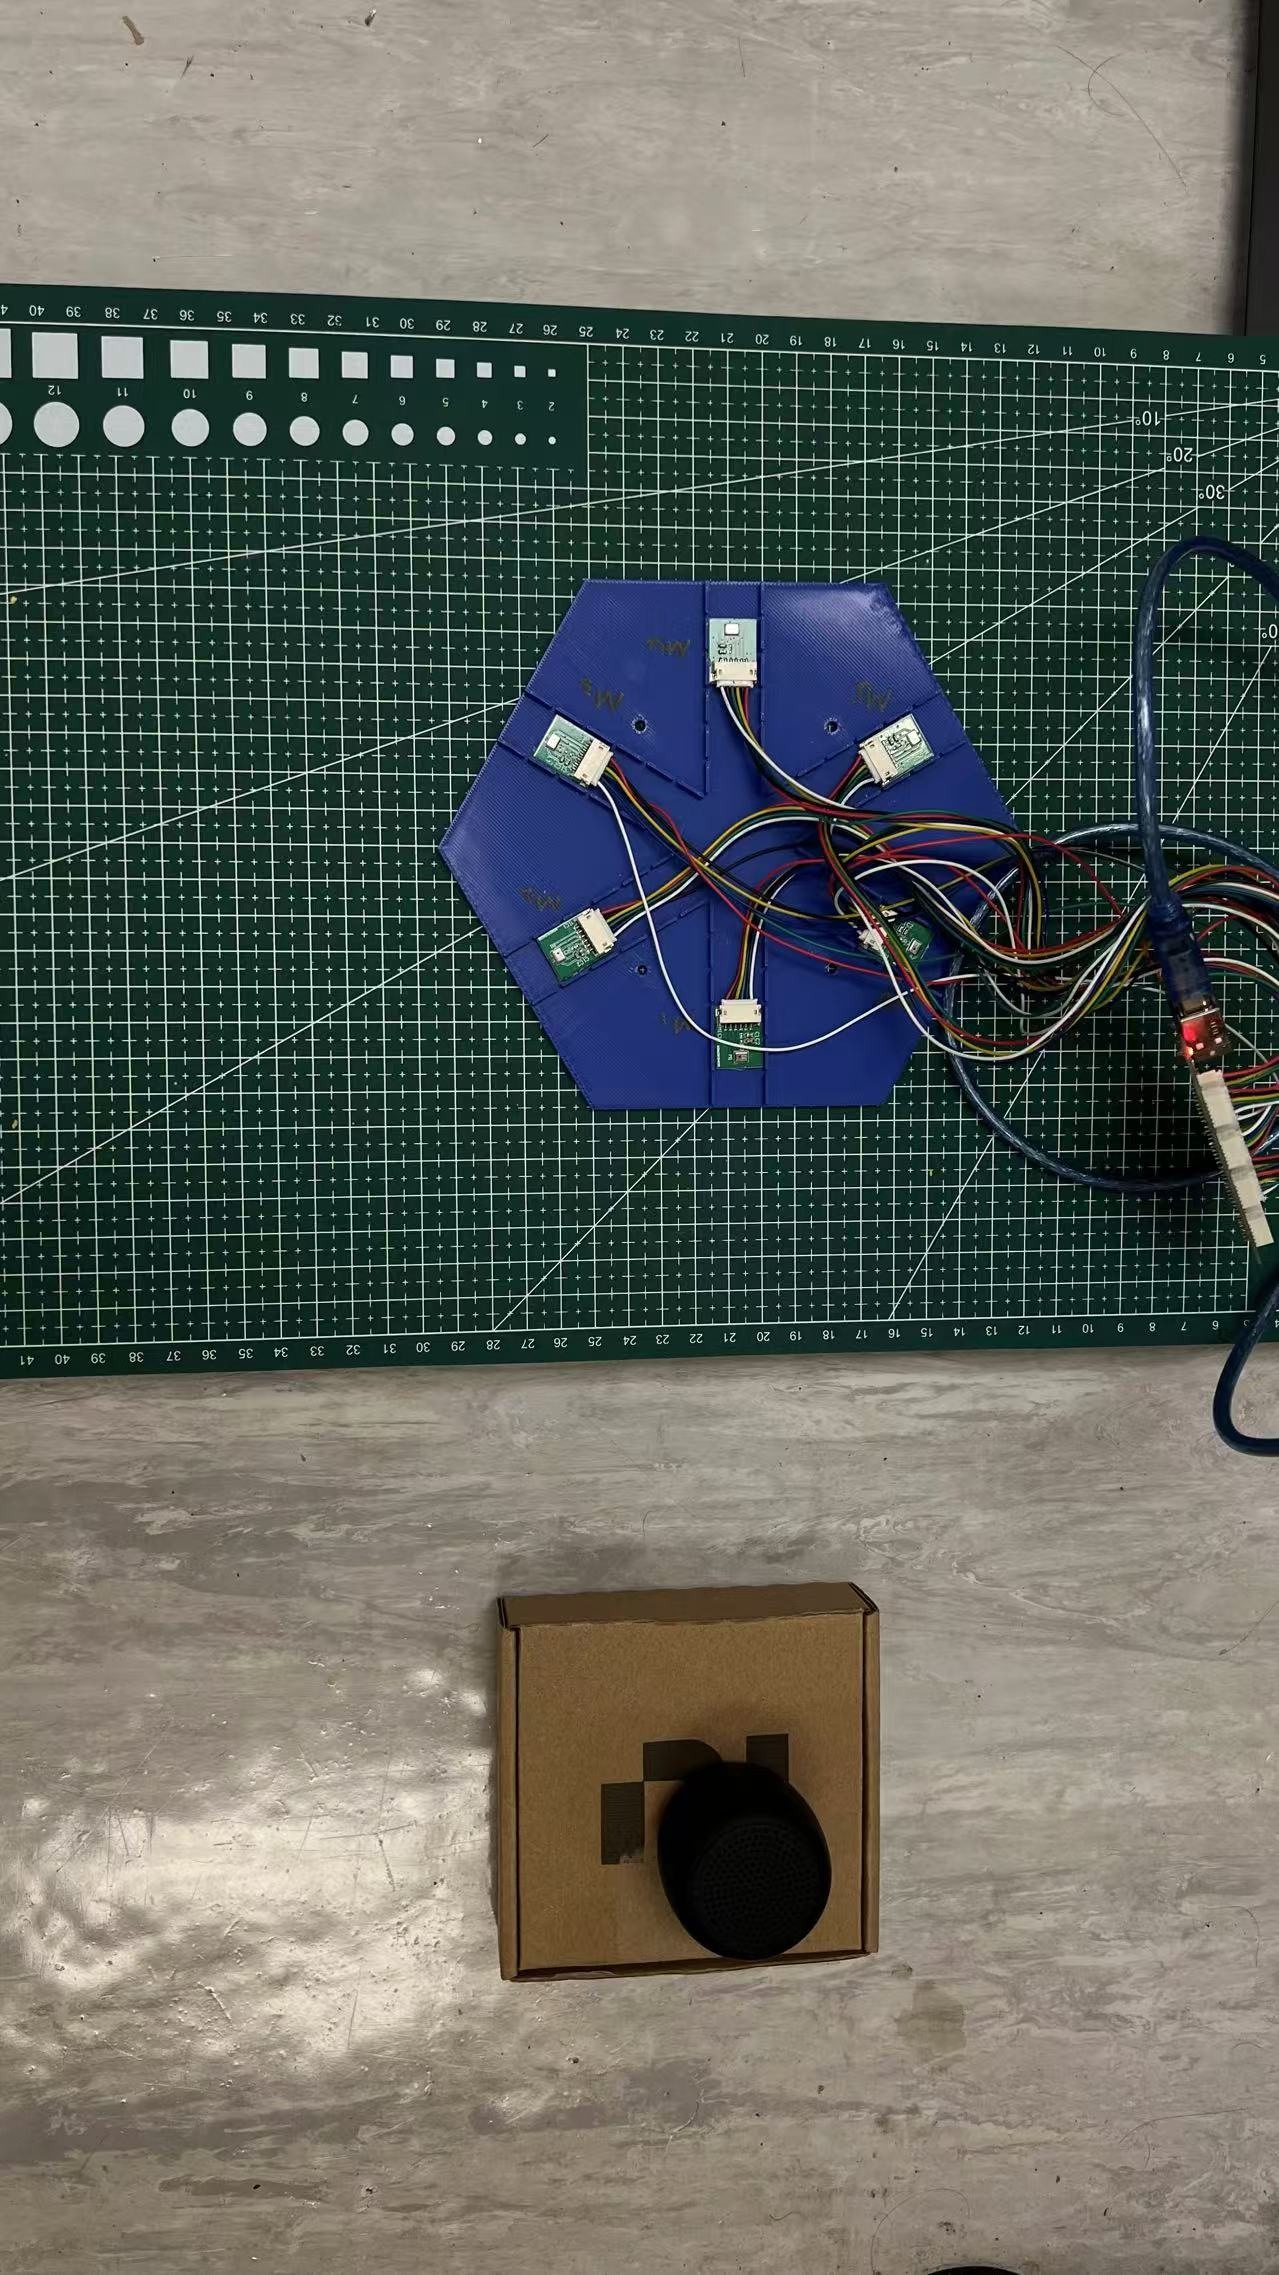
\includegraphics[width=0.5\linewidth]{figures/Microphone_array_photo_2.jpg}}
        \end{minipage}
        \caption{Hexagonal Microphone Array Apparatus}
    \end{figure}
\end{enumerate}

The setting of the SSL scenario is tentatively described by the following:
\begin{enumerate}
    \item The sound source is located \(0.3m\) to \(2m\) from the center of the microphone array. It is a blue-tooth speaker playing a human-speaking voice segment from the Librispeech dataset \cite{panayotov_resource_2015}.
    \item The sound source is located in the front of the microphone array, with its range of angle defined as \(\theta \in [0, \pi]\) in radius or \(\theta_d \in [0, 180]\) in degree. The unit circle defines the angle's orientation, which is counter-clockwise starting from the positive direction of the x-axis.
        
    \begin{figure}[H]
        \centering
        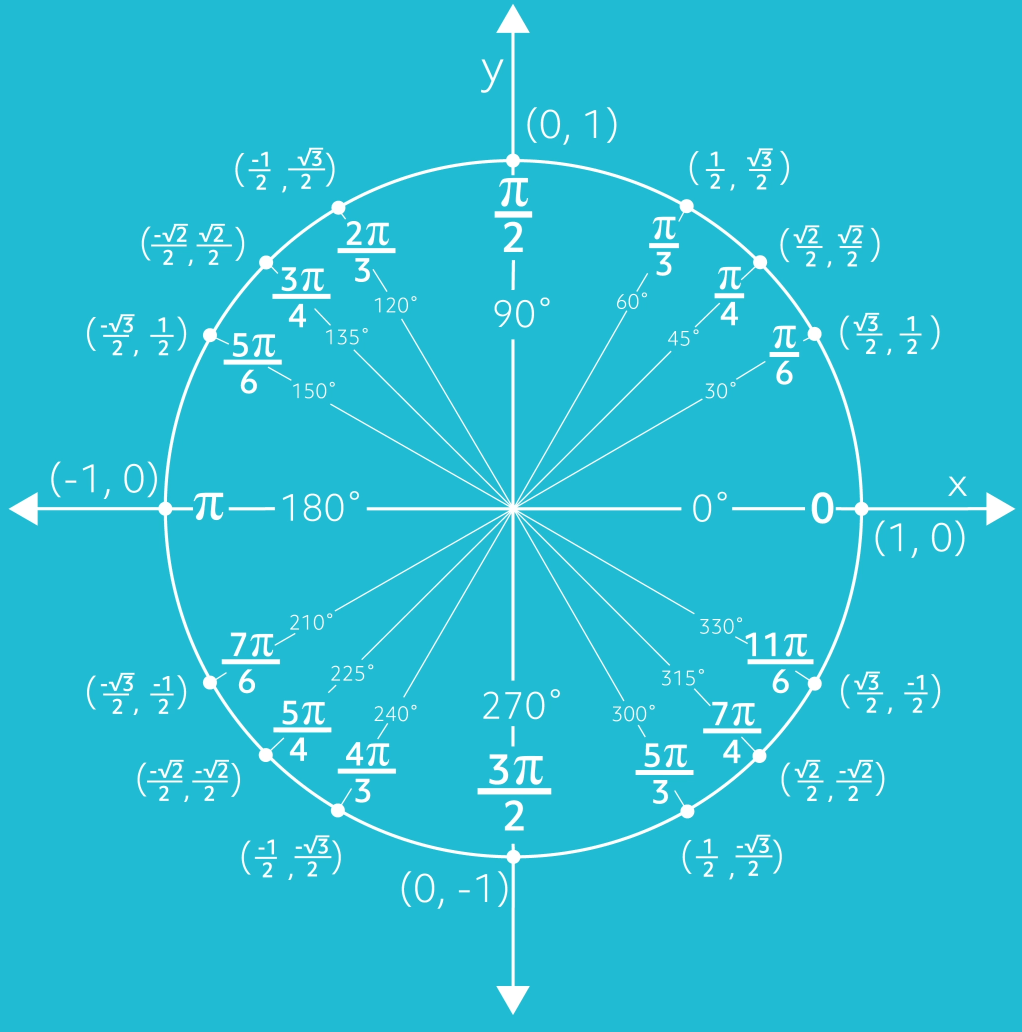
\includegraphics[width=0.3\linewidth]{figures/Unit_circle.png}
        \caption{Unit Circle}
    \end{figure}
    \item The distance between the center of the microphone array and the sound source is relatively large compared to the distances between microphones in the microphone array, indicating that the situation of the microphone array surrounding the sound source will not be considered.
    \item The surrounding environment is defined to be an indoor environment, indicating that complicated outdoor noises will not be involved. The non-reverberant situation will be first tested by utilizing the anechoic chamber. Future studies may include the reverberant situation if sufficient time exists.
    \item The input of the algorithm is defined as a ".wav" audio file, which will be further converted into two data:
    \begin{itemize}
        \item The sample rate of the audio file is expressed as \(f_s\) in \(Hz\), denoting the number of samples per second.
        \item The original multi-channel sound signal represented as a matrix:
        \[
            \mathbf{S} = 
            \begin{bmatrix}
                s_1(t)\\
                s_2(t)\\
                \vdots\\
                s_6(t)\\
            \end{bmatrix}
        \]
        In reality, it is represented in discrete form:
        \[
            \mathbf{S} = 
            \begin{bmatrix}
                s_{1,1} & s_{1,2} & \cdots & s_{1,t*f_s} \\
                s_{2,1} & s_{2,2} & \cdots & s_{2,t*f_s} \\
                \vdots & \vdots & \ddots & \vdots \\
                s_{6,1} & s_{6,2} & \cdots & s_{6,t*f_s} \\
            \end{bmatrix}
        \]
        where \(t\) stands for the total time of this audio file. The amplitude is represented by \(s_{c,n} \in [-32767, 32768]\), using the PCM16 audio file coding format.
        
    \end{itemize}
    \item The output of the algorithm should be the degree of arrival (DoA) on the plane of the microphone array, which is defined as the Azmith angle \(\theta\). The sound source is assumed to be located on the same plane of the array. The elevation angle will not be considered in this project.

\end{enumerate}

Notice that this is a tentative setting. Further adjustments may be included during future experiments if the developed algorithm demonstrates high robustness, accuracy, and performance.


\section*{Traditional SSL Methods (XIAO Pengbo)}
\addcontentsline{toc}{section}{Traditional SSL Methods (XIAO Pengbo)}


TDOA (Time Difference of Arrival) method, as one of the classic SSL (Sound Source Localization) method, performs excellently in environments with low noise and low reverberation. Its principle involves triangulating the position based on the time differences in the arrival of signals.

Assuming a system composed of two microphones located at coordinates \((x_1, y_1)\) and \((x_2, y_2)\), with the speed of sound in the current environment being \(c\). When a sound is emitted from the source and received by the two microphones, the TDOA value obtained is \(t_{12}\). Multiplying the TDOA value by \(c\) gives the distance difference between the sound source and the two microphones. Based on this, we can solve for the coordinates of the sound source:
\[
\sqrt{(x-x_{1})^{2}+(y-y_{1})^{2}}-\sqrt{(x-x_{2})^{2}+(y-y_{2})^{2}}=c*t_{1-2}
\]
Solving this equation, the result is a hyperbola representing all possible locations of the sound source under TDOA. By adding a third point, the intersection of two hyperbolas allows us to accurately determine the position of the sound source.\\
\begin{figure}[H]
    \centering
    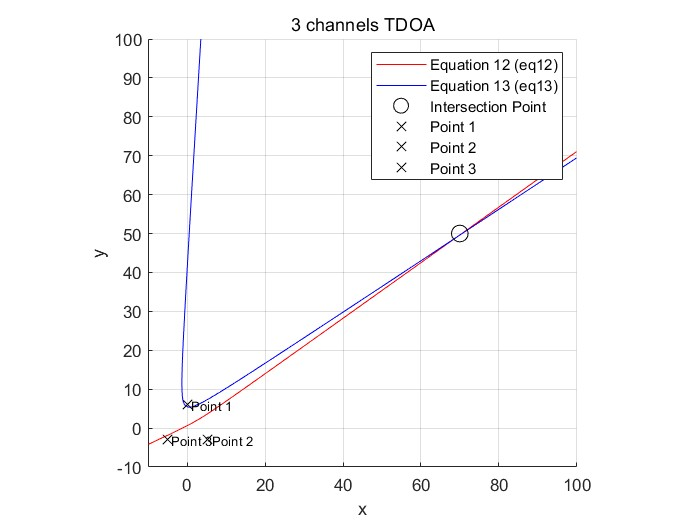
\includegraphics[width=0.7\linewidth]{figures/3_Channels.jpg}
    \caption{3-Channel TDOA Localization Schematic Diagram}
\end{figure}
Generally, there are two ways to obtain TDOA values: 

The first method involves subtracting the time of arrival (TOA) at each receiver. The limitation of this approach is that acquiring TOA requires strict synchronization between the signal source and the receivers. Therefore, this method is not suitable for locating randomly occurring signal sources in an environment.

The second method involves performing correlation calculations on the signals received by two receivers to obtain the TDOA value. This method does not require time synchronization between the sound source and the receivers, making it applicable in a wider range of scenarios and suitable for processing sporadic sound information in the environment. Therefore, this project employs the second method to solve for the TDOA value. 

In our project, the specific methods and principles are as follows:
\begin{enumerate}
    \item Collecting the sound pressure signals from each receivers while ensure all the receivers are time-synchronized. The signals are represented as the following matrix:
    \[
        \mathbf{S} = 
        \begin{bmatrix}
            s_1(t)\\
            s_2(t)\\
            \vdots\\
            s_6(t)\\
        \end{bmatrix}
    \]
    \(s_1\) to \(s_6\) is the signals of 6 channels (according to \textit{ The Geometry of the Hexagonal Microphone Array}, corresponding to M1 through M6).
    \item The project team divides the microphone array into 2 groups: M1 M3 M5 and M2 M4 M6. These two sets of signals, based on M1 and M2, are used for GCC (Generalized Cross-Correlation) calculation. The detail calculations are as following:
    
\end{enumerate}



\section*{Deep-Learning Based SSL Methods (ZENG Bailin)}
\addcontentsline{toc}{section}{Deep-Learning Based SSL Methods (ZENG Bailin)}


The SSL problem is defined as a classification problem instead of a regression problem. The algorithm input should be the original sound signal. The output of the DNN should be an array, with 180 elements representing the corresponding probability of DoA.\\
Notice that the development of the SSL deep learning model's structure is based on a current research project, \textit{Trusted Sound Source Localization} \cite{devin_sound_2024}.

\subsection*{Short-time Fourier Transform}
\addcontentsline{toc}{subsection}{Short-time Fourier Transform}
The feature extraction part Learning (DL) approach for sound source localization uses the Short-time Fourier Transform (STFT) projecting the time-domain multi-channel signal \(S\) to the time-frequency domain in the form of a spectrogram and processing the spectrogram using DNN. The STFT retains the audio signal variation with respect to time, as this variation may affect the result of the localization process. \\
The mathematical expression of the STFT is described as:
\[
    \textbf{STFT}_c(s_c(t), t,f) = \int_{-\infty}^{\infty} w(t-\tau) s_c(\tau) e^{-j2\pi f\tau}d\tau 
\]
where:
\begin{itemize}
    \item \(c\) is the index of microphone.
    \item \(w\) is a windowed function separating each time frame segment.
    \item \(t, f\) is the time and frequency in the final time-frequency domain. 
\end{itemize}
The discrete implementation of the STFT usually involves using the Fast Fourier Transform (FFT) to implement the transformation:
\[
    \textbf{STFT}_c(s_{c,n}, t, f) = \sum_{n = 1}^{N} s_{c,n} w(n-t) e^{-i2\pi k \frac{n}{N}}
\]
where:
\begin{itemize}
    \item \(s_{c,n}\) is the sample of the audio signal in channel \(c\) and sample index \(n\).
    \item \(N\) is the total number of samples, which should be \(N = t * f_s\).
\end{itemize}
Notice that in the application, this process is in discrete form, using summation instead of integration.
The resulting spectrogram is a time-frequency domain containing complex numbers, which contains the real part representing the amplitude, and the imaginary part representing the phase shift. Expressing in the form of a 3-dimensional tensor: \(\mathbf{X}_{ctf}\), where \(c\) is current microphone channels, \(f\) is frequency bin, and \(t\) is time frame.

However, during the implementation of the deep-learning process, the model should be able to understand the connection between the amplitude and phase shift for each time-frequency segmentation. Therefore, the imaginary parts are extracted from the original tensor \(\mathbf{X}_{ctf}\), transformed into real numbers, and concatenated along the channel dimension. The final shape of the resulting tensor, which is also the direct input of the DNN, should be:
\[
    \mathbf{X} \in \mathbb{R}^{2C\times F \times T}
\]
where \(C\) is the total number of microphone channels, \(F\) is the total number of frequency bins, and \(T\) is the total number of time frame.


\subsection*{Structure of the Deep-neural Network}
\addcontentsline{toc}{subsection}{Structure of the Deep-neural Network}
The structure of the DNN to process the result of STFT utilizes a combination of several structures, including Causal Convolution layers, 2-dimensional Max Pooling Layers,  Long short-term memory structure, and a fully connected layer. 
Defining the input of the DNN as:
\[
    \mathbf{X} \in \mathbb{R}^{B \times 2C\times F \times T}
\]
where \(B\) is the batch size per each propagation for the model's training purpose.\\
Tentatively, the architecture of the DNN's forward propagation is designed as the following:
\[
    \textbf{CRNN}(\mathbf{X}) = \textbf{FC}(\textbf{RNN}(\textbf{CNN}(\mathbf{X})))
\]
\textbf{CNN} is a convolution block including one layer of multi-head attention, further extracting important features from the multi-channel spectrogram \(\mathbf{X}\) and ignoring the unrelated feature. This block is formed by repeated 2-dimensional convolution block and 2-dimensional max-pooling processes in the time and frequency dimensions, expressed as:
\begin{align*}
    \textbf{CNN}(\mathbf{X}) = \textbf{MaxPool2d}(\textbf{CnnBlock}(\textbf{MaxPool2d}(\textbf{MultiHeadAttention}( \\
    \underbrace{\textbf{MaxPool2d}(\textbf{CnnBlock}(\ldots \textbf{CnnBlock}(\mathbf{X})\ldots}_{\text{3 times}}))))
\end{align*}
where the \textbf{MaxPool2d} is a 2-dimensional pooling layer, extracting the maximum number in a kernel. The \textbf{MultiHeadAttention} is a multi-head attention layer, correlating the information across the frequency dimension so that the model can comprehend information across different frequency bins.
The structure of the \textbf{CnnBlock} is given by:
\[
    \textbf{CnnBlock}(\mathbf{x}) = \textbf{Conv2d}(\textbf{BN}(\textbf{ReLU}(\textbf{Conv2d}(\mathbf{x})))
\]
where \textbf{Conv2d} is a standard 2-dimensional convolution layer, and \(\mathbf{x}\) is the output from the previous block and input of that block. \textbf{BN} is the batch normalization process, normalizing all the data along the batch dimension. \textbf{ReLU} is the rectified linear unit activation function.\\
The \textbf{RNN} is a standard long short-term memory layer (LSTM). Before entering the \textbf{RNN} layer, the tensor will be reshaped into a 3-dimensional tensor, and the frequency and channel dimensions will be combined:
\[
    \textbf{CNN(X)} = \mathbf{X}_{cnn,out} \in \mathbb{R}^{B \times 2C\times F' \times T'} \rightarrow \mathbf{X}_{rnn,in} \in \mathbb{R}^{B \times T' \times (F' \times 2C)}
\]
where the \(T'\) and \(F'\) are the total time frame and frequency bins after the \textbf{CNN} block. With the aid of the LSTM, the DNN should be able to comprehend the signal changes across the time frame. In case there are positional changes in the sound source, the model can correlate the sound source's position in the current time frame to the previous time frame. Meanwhile, through this LSTM process, the output dimension will be settled to 180:
\[
    \textbf{RNN}(\mathbf{X}_{rnn,in}) = \mathbf{X}_{rnn,out} \in \mathbb{R}^{B \times T' \times 180}
\]
The last layer of the model, the \textbf{RC}, is a fully connected layer, with its structure given by:
\[
    \mathbf{X}_{output} \in \mathbb{R}^{B \times T' \times 180} = \textbf{RC}(\mathbf{X}_{rnn,out}) = \textbf{Linear}(\textbf{Dropout}(\mathbf{X}_{rnn,out}))
\]
where the \textbf{Dropout} layer randomly discards data in neurons to prevent the over-fitting of the model, and the \textbf{Linear} layer is a linear mapping to the final output. The final output has three dimensions: the \(B\) is the batch size, \(T'\) is the convoluted time frames (the predicted time step), and \(180\) is the classes representing 180 degrees. The final resulting data is \(p \in \mathbb{R}\) representing the possibilities of sound sources existing in each class and each predicted time step.\\


\subsection*{Loss}
\addcontentsline{toc}{subsection}{Loss}
The loss function is crucial for the evaluation of the model's performance. The function takes in the predicted result and labels ground truth as inputs, and outputs the loss value representing the correctness of the prediction. It is used for the gradient descending process for the DNN training to adjust its parameters to approximate the ground truth, generating more trustworthy results.\\
In this DNN model, given the predicted output:
\[
    x_{b,t,c} = \mathbf{X}_{output} \in \mathbb{R}^{B \times T' \times 180} 
\]
and the labeled ground truth:
\[
    \mathbf{GT} \in \mathbb{R}^{B \times T'}
\]
where in each section of \(\mathbf{GT}\) there exists a DoA in radius representing the true DoA.\\
The cross-entropy function is used as the loss function. It involves several steps:
\begin{enumerate}
    \item Transform the ground truth from radius to degree:
    \[
        \text{GroundTruth}_{b,t} = \mathbf{GT}_{deg} = \mathbf{GT} \frac{180}{\pi}
    \]
    \item Generate truth label from the \(\mathbf{GT_{deg}}\):
    \[
        \text{one hot}(\mathbf{GT_{deg}}) = t_{b,t,c} = 
        \begin{cases}
        1 & \text{if } c = \text{GroundTruth}_{b,t}\\
        0 & \text{if } c \neq \text{GroundTruth}_{b,t}\\
        \end{cases}
        =\mathbf{T} \in \mathbb{R}^{B \times T' \times 180}
    \]
    where the result tensor \(\mathbf{T}\) has '1' for the correct class in each time frame, and '0' for each incorrect class.
    \item Apply the cross-entropy function to get the final loss for each time frame:
    \[
        loss_{b,t} = -\sum_{i = 1}^{180} t_{b,t,i} \log (x_{b,t,i}) = \mathbf{L} \in \mathbb{R}^{B \times T'}
    \]
\end{enumerate}

\subsection*{Prediction of DoA}
\addcontentsline{toc}{subsection}{Prediction of DoA}
Once the predicted tensor \(x_{b,t,c}\) is gained, the final prediction of DoA is given by:
\[
    \text{PredDoA}_{b,t} = \text{argmax}(x_{b,t,c}, \text{dim} = 2)
\]
The index of the class among the 180 classes will be returned for each batch and each time frame denoted as the DoA of prediction.\\

\subsection*{Computational Data Generation}
\addcontentsline{toc}{subsection}{Computational Data Generation}
The initial training process of the DNN utilizes computationally generated data, which can be gained at a lower cost than real-time recording. Meanwhile, different acoustic scenarios can be simulated by using the \textit{gpuRIR} \cite{diaz-guerra_gpurir_2021} and \textit{webrtcVAD} python libraries. During the data generation process, clean voice data from \textit{LibriSpeech} \cite{panayotov_resource_2015} will be segmented and integrated with noises from the dataset \textit{Noise92} \cite{andrew_assessment_1993}. The \textit{webrtcVAD} library is utilized to detect whether the segmentation contains noise, removing the empty segment from the dataset. The \textit{gpuRIR} \cite{diaz-guerra_gpurir_2021} is utilized to simulate the sound transmission process, generating the final signal received by each microphone channel. The \textit{gpuRIR} \cite{diaz-guerra_gpurir_2021} can also be used to simulate room reverberation and high reverberant cases will be considered in future testing if the model can process the non-reverberation case properly.\\
During the data generation process, the DoA will be selected randomly, and the clean voice segmentation and noise will be used to ensure the model adapts to various acoustic situations.\\
Three datasets will be generated: one for the training of the DNN, one for accuracy validation after each training epoch, and one for the final testing of the model's performance.

\subsection*{The Training Process}
\addcontentsline{toc}{subsection}{The Training Process}
All the parameters in the previously mentioned structures are to be changed during the model training process, which uses labeled ground truth and the backward propagation process to adjust these parameters to fit the training data. \\
The entire training process will be divided into epochs, and each epoch will be divided into steps. During one epoch, the DNN will process all the labeled data in the training dataset and a validation process will be conducted at the end of the one epoch, using the validation dataset to verify the result of this epoch. For each step, one batch, containing the number of data equal to the batch size, will be processed once through the DNN, including forward propagation and backward propagation, and the parameters will be adjusted once at the end.\\
After a given number of epochs, the training process is regarded as finished, and the testing dataset will be used to measure the prediction performance of the model.


\section*{Mobile Platform (WU Zhuoli)}
\addcontentsline{toc}{section}{Mobile Platform (WU Zhuoli)}

\input{chapters/methodology/mobile_platform}
\chapter*{Experiments}
\addcontentsline{toc}{chapter}{Experiments}

In this section, experiments that were conducted for each part of the project will be described, including the experiment settings and the data collected. The experiments described only include the experiments conducted before the submission of this Interim Report, excluding the future experiments plan.



\section*{Traditional SSL Methods (XIAO Pengbo)}
\addcontentsline{toc}{section}{Traditional SSL Methods (XIAO Pengbo)}


TDOA (Time Difference of Arrival) method, as one of the classic SSL (Sound Source Localization) method, performs excellently in environments with low noise and low reverberation. Its principle involves triangulating the position based on the time differences in the arrival of signals.

Assuming a system composed of two microphones located at coordinates \((x_1, y_1)\) and \((x_2, y_2)\), with the speed of sound in the current environment being \(c\). When a sound is emitted from the source and received by the two microphones, the TDOA value obtained is \(t_{12}\). Multiplying the TDOA value by \(c\) gives the distance difference between the sound source and the two microphones. Based on this, we can solve for the coordinates of the sound source:
\[
\sqrt{(x-x_{1})^{2}+(y-y_{1})^{2}}-\sqrt{(x-x_{2})^{2}+(y-y_{2})^{2}}=c*t_{1-2}
\]
Solving this equation, the result is a hyperbola representing all possible locations of the sound source under TDOA. By adding a third point, the intersection of two hyperbolas allows us to accurately determine the position of the sound source.\\
\begin{figure}[H]
    \centering
    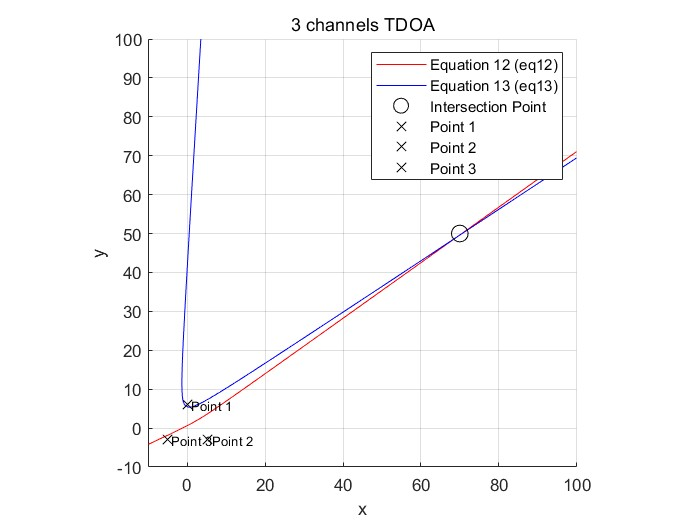
\includegraphics[width=0.7\linewidth]{figures/3_Channels.jpg}
    \caption{3-Channel TDOA Localization Schematic Diagram}
\end{figure}
Generally, there are two ways to obtain TDOA values: 

The first method involves subtracting the time of arrival (TOA) at each receiver. The limitation of this approach is that acquiring TOA requires strict synchronization between the signal source and the receivers. Therefore, this method is not suitable for locating randomly occurring signal sources in an environment.

The second method involves performing correlation calculations on the signals received by two receivers to obtain the TDOA value. This method does not require time synchronization between the sound source and the receivers, making it applicable in a wider range of scenarios and suitable for processing sporadic sound information in the environment. Therefore, this project employs the second method to solve for the TDOA value. 

In our project, the specific methods and principles are as follows:
\begin{enumerate}
    \item Collecting the sound pressure signals from each receivers while ensure all the receivers are time-synchronized. The signals are represented as the following matrix:
    \[
        \mathbf{S} = 
        \begin{bmatrix}
            s_1(t)\\
            s_2(t)\\
            \vdots\\
            s_6(t)\\
        \end{bmatrix}
    \]
    \(s_1\) to \(s_6\) is the signals of 6 channels (according to \textit{ The Geometry of the Hexagonal Microphone Array}, corresponding to M1 through M6).
    \item The project team divides the microphone array into 2 groups: M1 M3 M5 and M2 M4 M6. These two sets of signals, based on M1 and M2, are used for GCC (Generalized Cross-Correlation) calculation. The detail calculations are as following:
    
\end{enumerate}



\section*{Deep-Learning Based SSL Methods (ZENG Bailin)}
\addcontentsline{toc}{section}{Deep-Learning Based SSL Methods (ZENG Bailin)}

The experiment conducted for the DL-based method before the interim report mainly contains the model training experiment, aiming to observe the model's stability of converging. The process of testing real-world data using this model will be conducted in the coming semester. In this section, the details of the DNN model training experiment will be described.\\
In the training process, the loss of each training epoch and the loss of the validation part at the end of each epoch were recorded. Meanwhile, at the end of each training process, the model's accuracy was evaluated.\\
Notice that for each model training process, a new dataset of audio received by a 6-channel microphone was computationally generated using the same parameter:
\begin{itemize}
    \item Original clean voice segmentation and noise segmentation selected randomly from the database.
    \item Signal to noise ratio randomly set between a range of values, such as between \(-5 db\) to \(15 db\).
    \item Location of the sound source randomly set between \(0.3m\) to \(1.5m\) from the center of the microphone array.
    \item Degree of arrival randomly set between \(0^{\circ}\) to \(180^\circ\).
\end{itemize}
Meanwhile, the validation dataset is generated using the same settings.\\

\subsection*{Performance Evaluation Metrics}
\addcontentsline{toc}{subsection}{Performance Evaluation Metrics}
Three metrics are used to measure the performance of the predicted result of the DNN:
\begin{enumerate}
    \item Loss of the prediction result.
    \item Mean Absolute Error (MAE) of predicted angle, given by:
    \[
        \text{MAE} = \frac{1}{(B\times T')} \sum_{i = 1}^{B}\sum_{j = 1}^{T'} |\text{GroundTruth}_{i,j}-\text{PredDoA}_{i,j}|
    \]
    where \(B\) is the total number of Batches, and \(T'\) is the time frame predicted in each batch.
    \item Accuracy (ACC) of the predicted angle, given by:
    \[
        \text{ACC} = \frac{\text{Number of Correct Predictions}}{\text{Total Number of Predictions}}
    \]
    The situations of \(|\text{GroundTruth}_{b,t}-\text{PredDoA}_{b,t}| < 5^\circ\) are considered as correct prediction.
\end{enumerate}

\subsection*{Batch Size Experiment}
\addcontentsline{toc}{subsection}{Batch Size Experiment}
An experiment is carried out to test the difference of the model training using various batch size settings. Three experiments were conducted using \(\text{batch size} = 4,8,16\) (our hardware does not allow us to use larger batch sizes such as \(32\)). The training results are attached to the \textit{The DL Experiment Result of Different Batch Sizes}.\\
The Following conclusions can be made:
\begin{itemize}
    \item All the experiments using various training batch sizes can converge, with final tested ACCs higher than \(0.95\).
    \item The tested results for the loss denote that varying batch size has a minor effect on the final training losses since all three experiments have final losses of approximately \(2.6\).
    \item The lowest MAE, a number of \(2.937\), appears when the batch size is \(8\), denoting that when batch size is \(8\), the prediction results are more concentrated.
\end{itemize}
A batch size of \(8\) should be chosen for the coming real-world audio processing experiment.

\subsection*{Mobile Sound Source and SNR Ranges Experiment}
\addcontentsline{toc}{subsection}{Mobile Sound Source and SNR Ranges Experiment}
Another experiment is conducted to test the model's performance when the sound source is mobile (noted as the sound source's status), meaning that the location of the sound source varies during the audio segmentation, or with different scales of SNR ranges, meaning that the range of noisiness of the audio. \\
Three cases were tested: a static sound source with a large SNR range, a mobile sound source with a large SNR range, and a static sound source with a small SNR range. The experiment results are attached in the appendix section \textit{The DL Experiment Result of Different Sound Source Status and SNR Ranges}. \\
The following conclusions can be made:
\begin{itemize}
    \item All three experiments have converging results except that the experiment \textit{Nov 3} has a slightly diverging trend after \(60\) epochs, denoting a possibility of over-fitting in that model. 
    \item It can be observed from the diagram that the training process of experiment \textit{Nov 6} is very unstable in epochs but demonstrates a better final testing result. It is possible this is a common phenomenon in DNN training due to randomness, including the random training data selection, random data dropout in the dropout layer, etc. 
    \item Comparing the difference between experiment \textit{Nov 3} and \textit{Nov 5}, it can be observed that Static sound source does not necessarily provide a more accurate prediction result since it has lower loss than mobile situation (denoting higher possibilities are predicted for the correct DoA) but has lower ACC than mobile situation (denoting a lower accuracy of prediction on the DoA with the highest possibilities).
    \item Comparing the difference between experiment \textit{Nov 5} and \textit{Nov 6}, it can be observed that a narrower range of SNR does provide a more accurate prediction result with lower loss, higher ACC, and lower MAE.
\end{itemize}
The model can comprehend both mobile sound sources and static sound sources. A narrower range of random SNR provides a more accurate prediction result.

\subsection*{Different SNRs Experiment}
\addcontentsline{toc}{subsection}{Different SNRs Experiment}
An experiment is conducted to test the model's performance when encountering different SNRs located in the same range. It is crucial to determine the effects on the prediction result of noisy audio. For the experiment, two settings are chosen: one with SNR ranging in \([1,10]db\), and the other with SNR ranging in \([30, 40]db\). The experiment results are attached in the appendix section \textit{The DL Experiment Result of Different SNRs}\\
The following conclusions can be made:
\begin{itemize}
    \item Increase in SNR has no effect on the maximum possible DoA predicted since both experiments have the same ACC.
    \item Increase in SNR has no effect on the divergence of DoA prediction error since both experiments have approximated MAE.
    \item An Increase in SNR does reduce the loss of prediction, denoting that the model provides more certainty of the predicted DoA compared with low SNR situations.
\end{itemize}





\section*{Mobile Platform (WU Zhuoli)}
\addcontentsline{toc}{section}{Mobile Platform (WU Zhuoli)}

\input{chapters/experiments/mobile_platform}

\chapter*{Conclusion}
\addcontentsline{toc}{chapter}{Conclusion}

% \section{Section}
% \subsection{Subsection}
% \subsubsection{Subsubsection}

% \printbibliography[heading = none]
\addcontentsline{toc}{chapter}{References}
\bibliographystyle{IEEEtran} % 设置参考文献样式
\renewcommand{\bibname}{References}
\bibliography{references.bib} % 指向BibTeX文件
\chapter*{Appendices}
\addcontentsline{toc}{chapter}{Appendices}

\section*{The Gantt Chart for Task Schedule}
\addcontentsline{toc}{section}{The Gantt Chart for Task Schedule}
\begin{figure}[H]
    \centering
    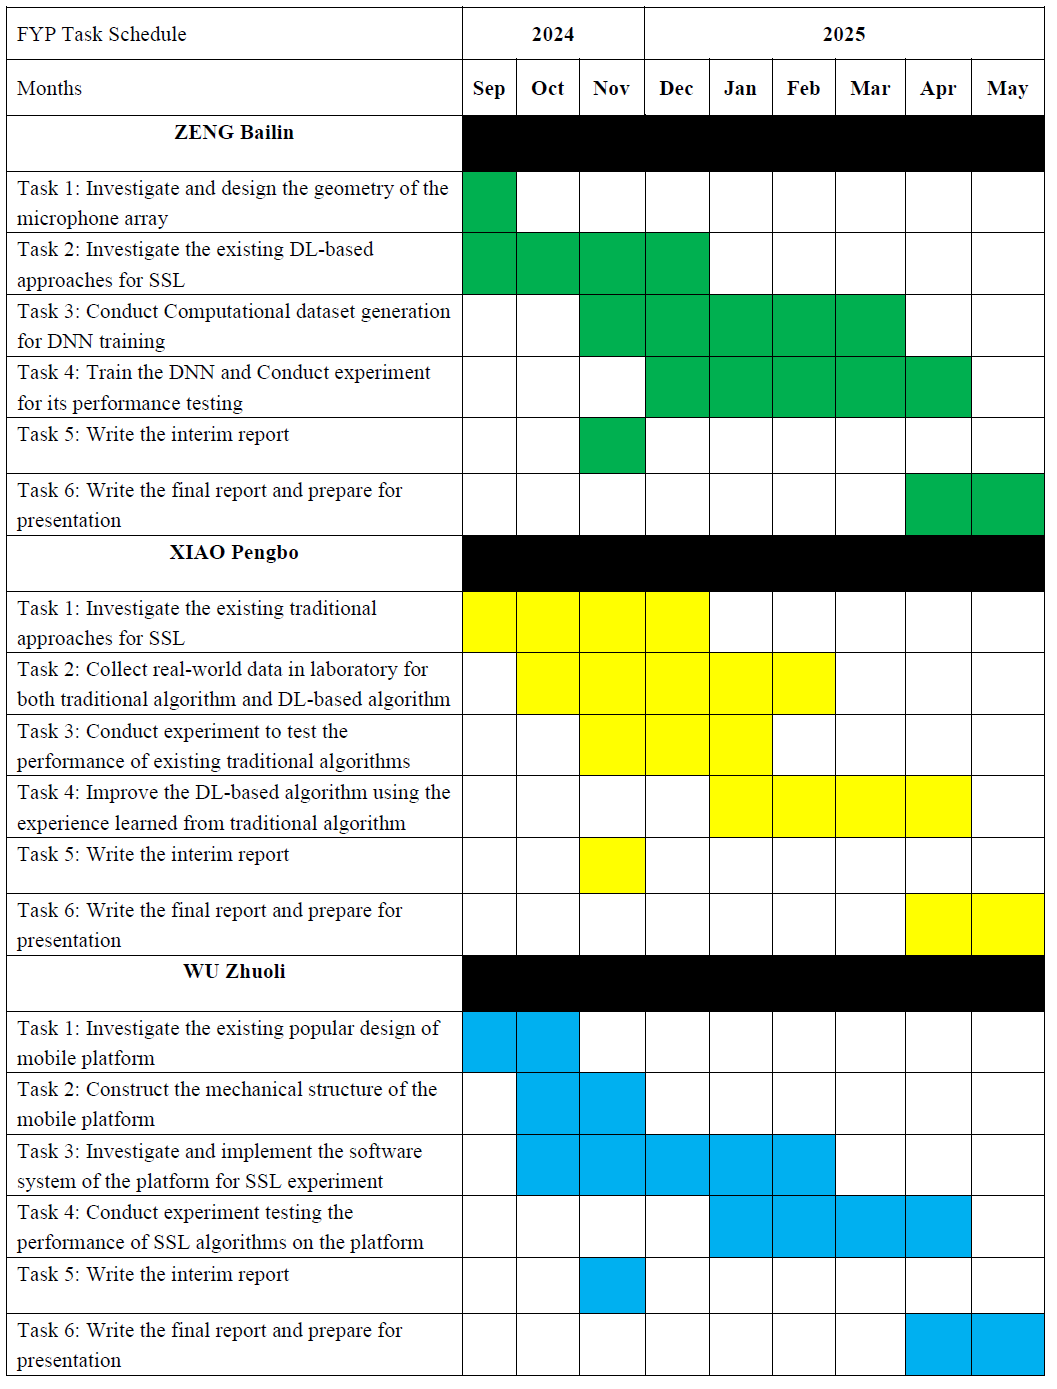
\includegraphics[width=1\linewidth]{figures/Gantt_chart.png}
\end{figure}



\section*{The DL Experiment Result of Different Batch Sizes}
\addcontentsline{toc}{section}{The Experiment Result of Different Batch Sizes}
\begin{figure}[H]
    \centering
    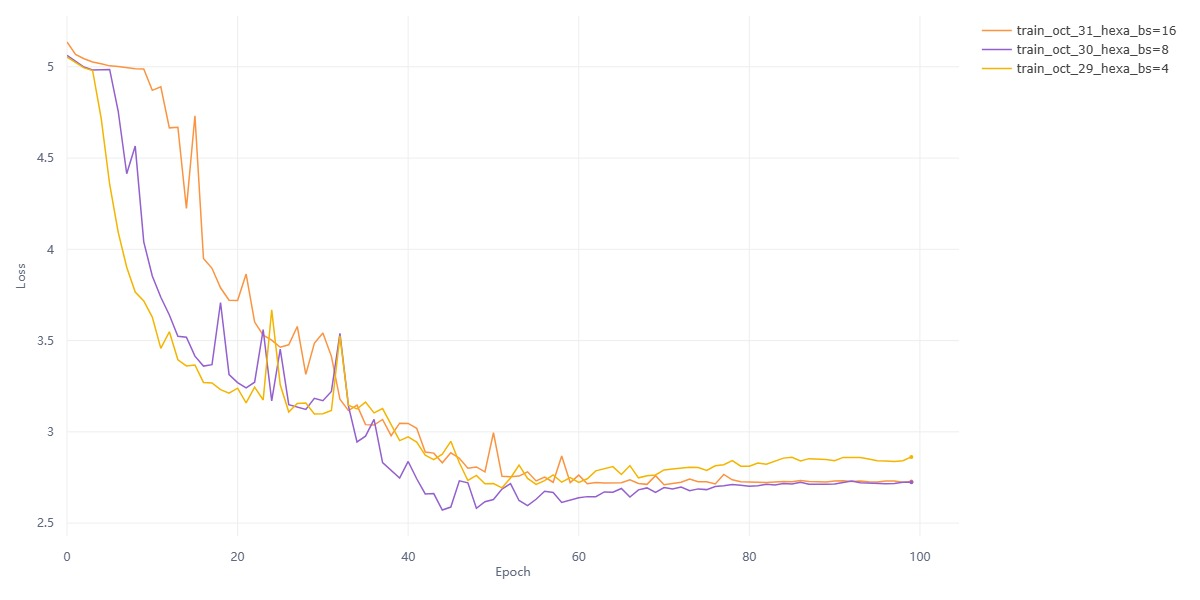
\includegraphics[width=1\linewidth]{figures/BS Valid_ Loss VS epoch.jpeg}
    \caption{Validation: Loss vs Epoch for Different Batch Sizes}
\end{figure}
\begin{figure}[H]
    \centering
    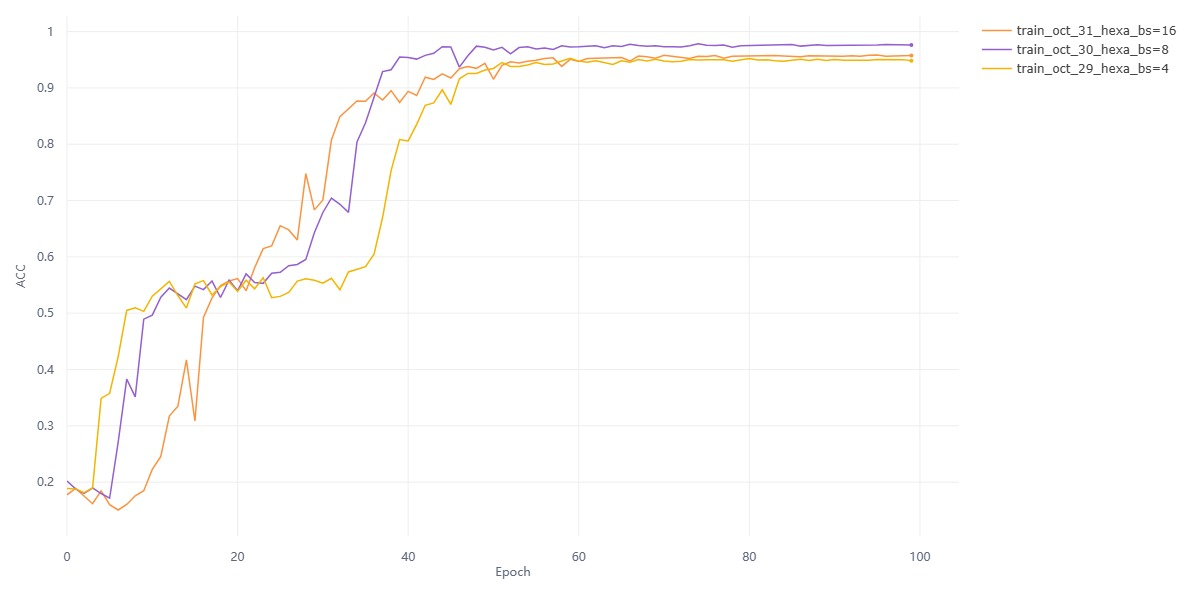
\includegraphics[width=1\linewidth]{figures/BS Valid_ ACC VS epoch.jpeg}
    \caption{Validation: ACC vs Epoch for Different Batch Sizes}
\end{figure}
\begin{figure}[H]
    \centering
    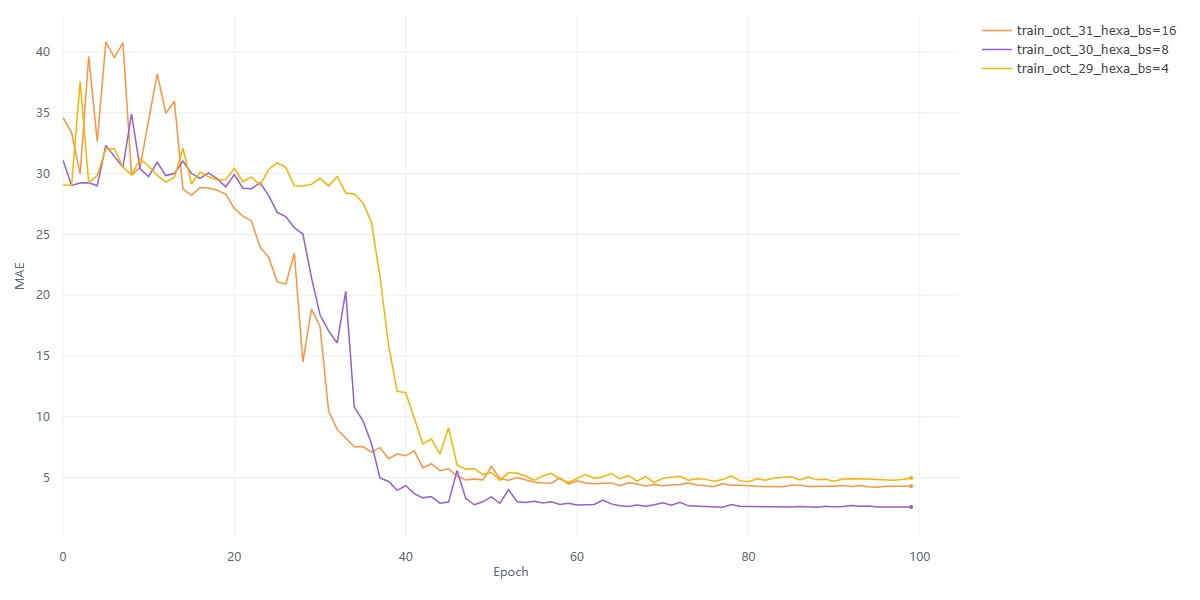
\includegraphics[width=1\linewidth]{figures/BS Valid_ MAE VS epoch.jpeg}
    \caption{Validation: MAE vs Epoch for Different Batch Sizes}
\end{figure}

\begin{table}[H]
    \centering
    \begin{tabular}{|c|c|c|c|c|}
        \hline
         Experiment Name& Batch Size & Test Loss & Test ACC & Test MAE\\
         \hline
         train oct 29 hexa bs=4& 4 & 2.719 & 0.9533 & 4.668\\
         \hline
         train oct 30 hexa bs=8& 8 & 2.592 & 0.9779 & 2.937\\
         \hline
         train oct 31 hexa bs=16& 16 & 2.638 & 0.9679 & 3.796\\
         \hline
    \end{tabular}
    \caption{Final Test Result of Different Batch Sizes}
\end{table}



\section*{The DL Experiment Result of Different Sound Source Status and SNR Ranges}
\addcontentsline{toc}{section}{The Experiment Result of Different Sound Source Status and SNR Ranges}
\begin{figure}[H]
    \centering
    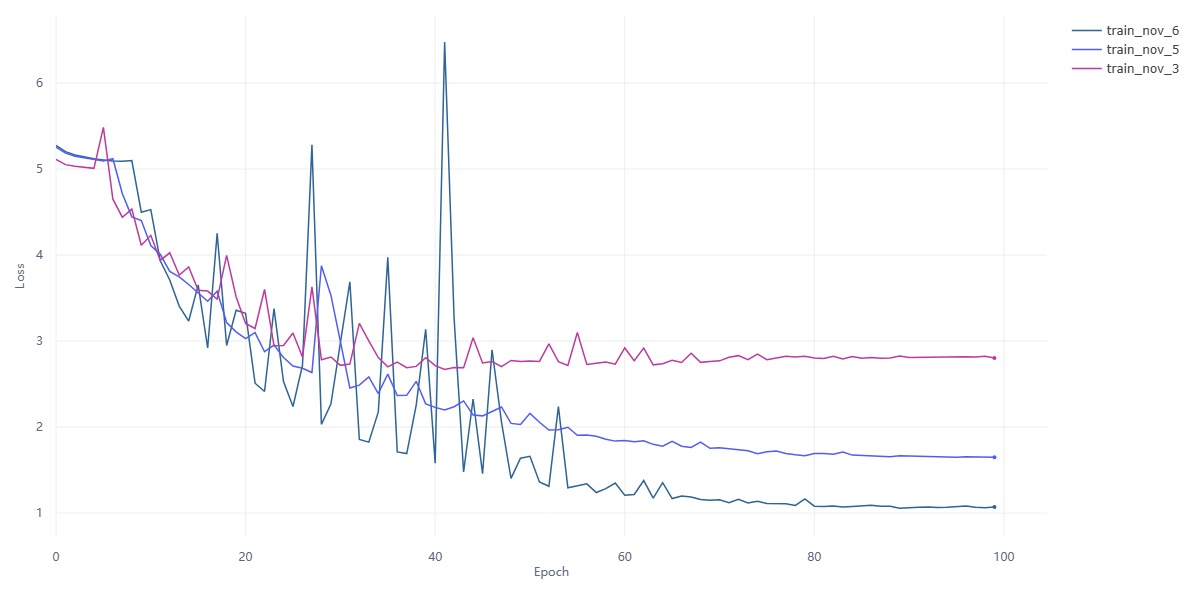
\includegraphics[width=1\linewidth]{figures/StatusSNR Valid_ Loss VS epoch.jpeg}
    \caption{Validation: Loss vs Epoch for Different Status and SNR Ranges}
\end{figure}
\begin{figure}[H]
    \centering
    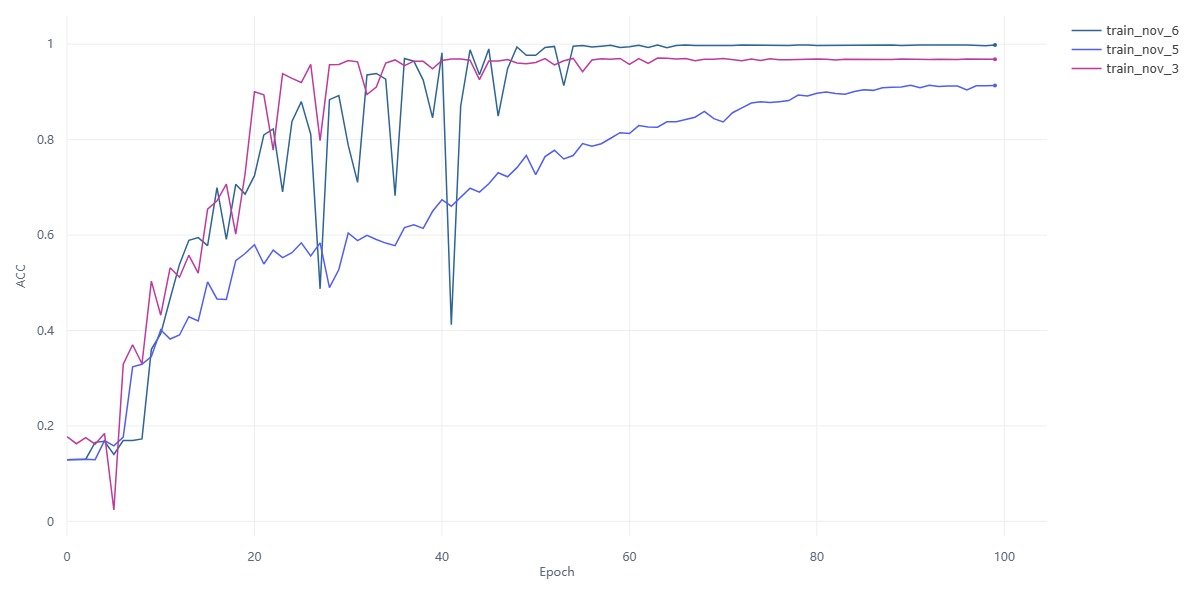
\includegraphics[width=1\linewidth]{figures/StatusSNR Valid_ ACC VS epoch.jpeg}
    \caption{Validation: ACC vs Epoch for Different Status and SNR Ranges}
\end{figure}
\begin{figure}[H]
    \centering
    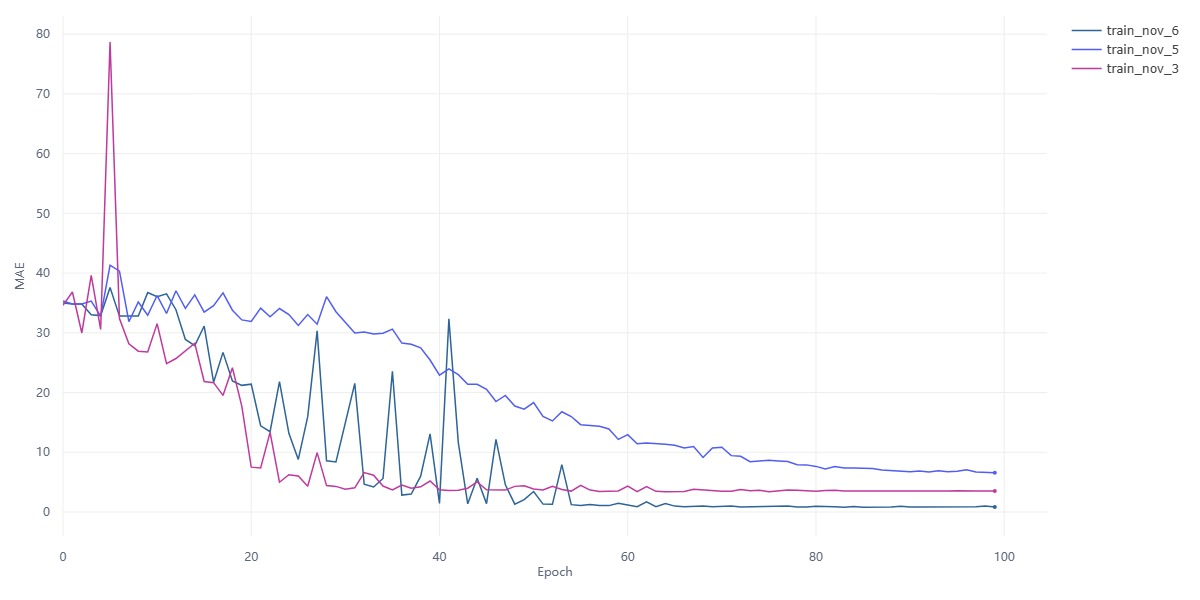
\includegraphics[width=1\linewidth]{figures/StatusSNR Valid_ MAE VS epoch.jpeg}
    \caption{Validation: MAE vs Epoch for Different Status and SNR Ranges}
\end{figure}
\begin{table}[H]
    \centering
    \begin{tabular}{|c|c|c|c|c|c|}
        \hline
         Experiment Name& Status & SNR (range in \(db\)) & Test Loss & Test ACC & Test MAE\\
         \hline
         train nov 3 & Mobile & \([-5, 15]\) & 2.731 & 0.9740 & 3.381\\
         \hline
         train nov 5 & Static & \([-5, 15]\) & 1.597 & 0.9145 & 5.568\\
         \hline
         train nov 6 & Static & \([1, 10]\) & 1.043 & 0.9988 & 0.789\\
         \hline
    \end{tabular}
    \caption{Final Test Result of Different Status and SNR Ranges}
\end{table}


\section*{The DL Experiment Result of Different SNRs}
\addcontentsline{toc}{section}{The Experiment Result of Different SNRs}
\begin{figure}[H]
    \centering
    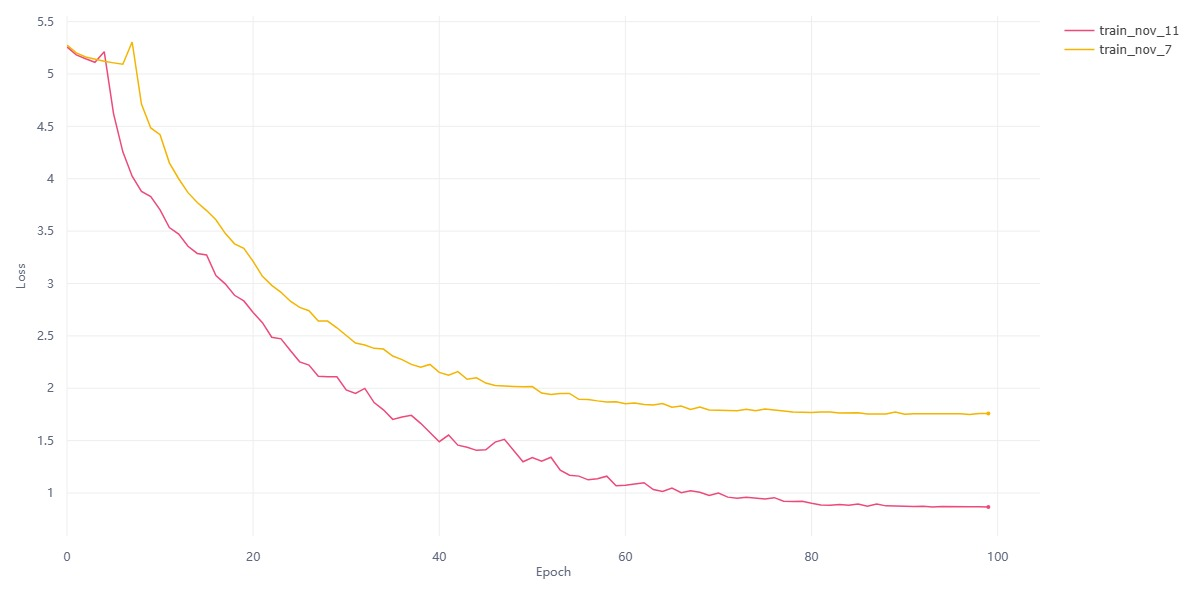
\includegraphics[width=1\linewidth]{figures/SNRs Valid_ Loss VS epoch.jpeg}
    \caption{Validation: Loss vs Epoch for Different SNRs}
\end{figure}
\begin{figure}[H]
    \centering
    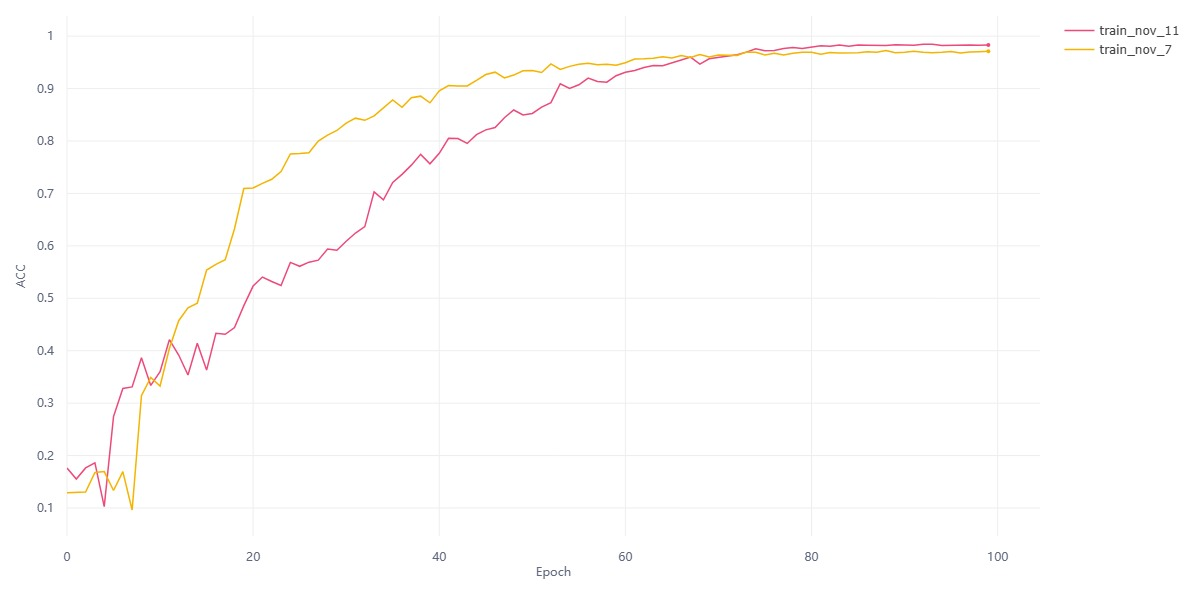
\includegraphics[width=1\linewidth]{figures/SNRs Valid_ ACC VS epoch.jpeg}
    \caption{Validation: ACC vs Epoch for Different SNRs}
\end{figure}
\begin{figure}[H]
    \centering
    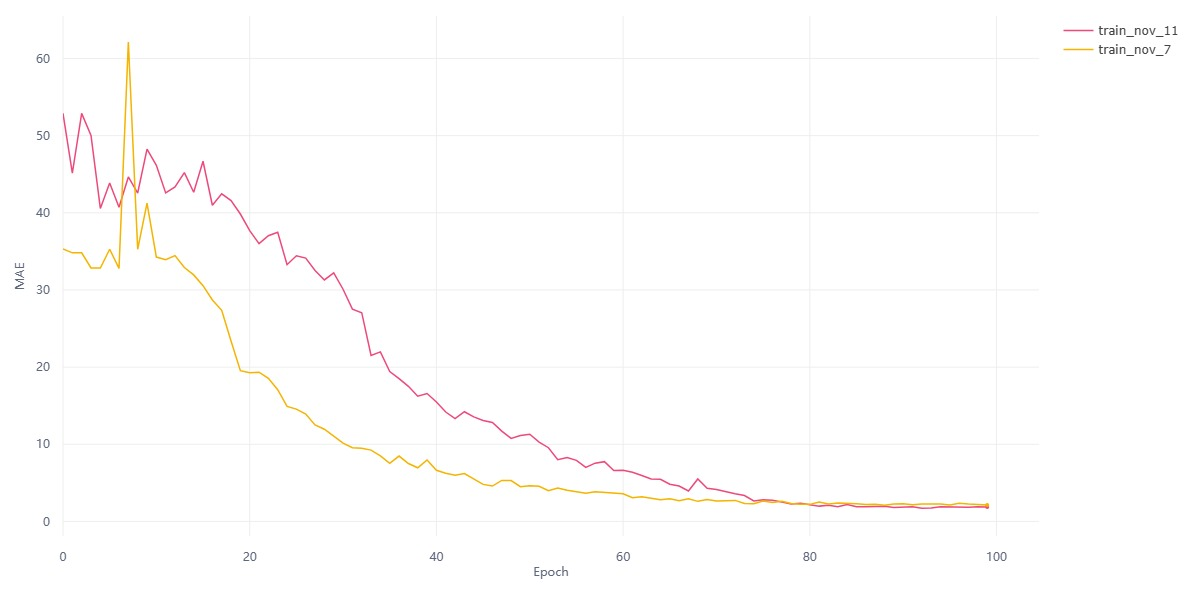
\includegraphics[width=1\linewidth]{figures/SNRs Valid_ MAE VS epoch.jpeg}
    \caption{Validation: MAE vs Epoch for Different SNRs}
\end{figure}
\begin{table}[H]
    \centering
    \begin{tabular}{|c|c|c|c|c|c|}
        \hline
         Experiment Name& SNR (range in \(db\)) & Test Loss & Test ACC & Test MAE\\
         \hline
         train nov 7 & \([1, 10]\) & 1.724 & 0.9723 & 2.198\\
         \hline
         train nov 1 & \([30, 40]\) & 0.8746 & 0.9772 & 2.38\\
         \hline
    \end{tabular}
    \caption{Final Test Result of Different SNRs}
\end{table}

\end{document}

